% !TEX program = pdflatex
% !TEX root = Bernal_H_JET_ES.tex
\documentclass[review,authoryear,12pt]{elsarticle}
\usepackage[T1]{fontenc}
\usepackage{times}
\usepackage{amssymb,mathtools,amsthm}

\RequirePackage[colorlinks,citecolor=blue,linkcolor=blue,urlcolor=blue,pagebackref]{hyperref}
\renewcommand*{\backref}[1]{}
\renewcommand*{\backrefalt}[4]{%
  \ifcase #1 %
  \or
    #2%
  \else
    #2%
  \fi
}
\renewcommand*{\backrefsep}{, }
\renewcommand*{\backreftwosep}{, }
\renewcommand*{\backreflastsep}{, }
\RequirePackage{float}
\RequirePackage{graphicx}
\RequirePackage{subcaption}
\captionsetup[figure]{skip=6pt}
\captionsetup[subfigure]{font=footnotesize,aboveskip=3pt,belowskip=2pt}
\setlength{\abovecaptionskip}{6pt}
\setlength{\belowcaptionskip}{4pt}
\setlength{\intextsep}{10pt plus 2pt minus 2pt}
\setlength{\textfloatsep}{16pt plus 2pt minus 4pt}
\setlength{\floatsep}{12pt plus 2pt minus 2pt}
\newlength{\subfigheight}
\setlength{\subfigheight}{4.2cm}
\newlength{\mapfigheight}
\setlength{\mapfigheight}{4.55cm}
\newlength{\widefigheight}
\setlength{\widefigheight}{3.4cm}
\newlength{\calfigheight}
\setlength{\calfigheight}{3.2cm}
\newlength{\calbeliefheight}
\setlength{\calbeliefheight}{4.5cm}
\newlength{\calseriesheight}
\setlength{\calseriesheight}{3.8cm}
\newlength{\calplotheight}
\setlength{\calplotheight}{4.2cm}
\newlength{\calpathheight}
\setlength{\calpathheight}{5.1cm}
\newcommand{\panelgraphic}[2]{%
  \parbox[t][#1][t]{\linewidth}{\centering\includegraphics[width=\linewidth,height=#1,keepaspectratio]{#2}}%
}
\newcommand{\figurenote}[1]{%
  \par\vspace{3pt}%
  \begingroup\footnotesize #1\par\endgroup
}
\RequirePackage{amsmath,amssymb,mathtools}
\RequirePackage{booktabs}
\RequirePackage{longtable}
\RequirePackage{tabularx}
\RequirePackage{array}
\RequirePackage{etoolbox}
\providecommand{\textcite}{\citet}

\graphicspath{{./Figures/}}


\theoremstyle{plain}
\newtheorem{theorem}{Teorema}
\newtheorem{proposition}[theorem]{Proposición}
\newtheorem{lemma}[theorem]{Lema}
\newtheorem{corollary}[theorem]{Corolario}

\theoremstyle{definition}
\newtheorem{definition}[theorem]{Definición}
\newtheorem{assumption}[theorem]{Supuesto}
\newtheorem{remark}[theorem]{Observación}

\newenvironment{fnnote}{%
  \begin{minipage}[t]{\linewidth}%
  \sloppy
}{\end{minipage}}

\newcommand{\thmendmark}{\par\nobreak{\hfill\ensuremath{\square}\par}}
\AtEndEnvironment{theorem}{\thmendmark}
\AtEndEnvironment{proposition}{\thmendmark}
\AtEndEnvironment{lemma}{\thmendmark}
\AtEndEnvironment{corollary}{\thmendmark}
\AtEndEnvironment{definition}{\thmendmark}
\AtEndEnvironment{assumption}{\thmendmark}
\AtEndEnvironment{remark}{\thmendmark}

\newcommand{\E}{\mathbb{E}}
\newcommand{\Prob}{\mathbb{P}}
\newcommand{\ProbE}{\mathbb{P}_{\mathrm{E}}}
\newcommand{\ProbC}[1]{\mathbb{P}_{\mathrm{C},#1}}
\newcommand{\ThetaK}{\Theta_K}
\newcommand{\TV}{\mathrm{TV}}
\newcommand{\dd}{\mathrm{d}}
\newcommand{\1}{\mathbf{1}}
\newcommand{\argmin}{\operatorname*{arg\,min}}
\newcommand{\argmax}{\operatorname*{arg\,max}}
\newcommand{\supp}{\operatorname{supp}}
\newcommand{\Dirac}{\delta}
\newcommand{\ProbI}[1]{\mathbb{P}_{\mathrm{I},#1}}
\newcommand{\Unif}{\mathrm{Unif}}



\renewcommand{\thetable}{\Roman{table}}
\renewcommand{\thefigure}{\Roman{figure}}
\providecommand{\doi}[1]{\href{https://doi.org/#1}{doi:\detokenize{#1}}}

% Plain, unboxed title-page layout (no "Abstract" heading, no horizontal
% rules) to match the Bernal_H.tex (econsocart) front page.
\makeatletter
\abstracttitle{}
% Tighter abstract box (no empty heading/medskip, reduced line spacing) so the
% abstract + keywords/JEL block fits on a single page together with the title.
\renewenvironment{abstract}{\global\setbox\absbox=\vbox\bgroup
  \hsize=\textwidth
  \linespread{0.92}\selectfont
  \noindent\ignorespaces}
 {\egroup}
\long\def\pprintMaketitle{\clearpage
  \iflongmktitle\if@twocolumn\let\columnwidth=\textwidth\fi\fi
  \resetTitleCounters
  \def\baselinestretch{1}%
  \printFirstPageNotes
  \begin{\elsarticletitlealign}%
 \thispagestyle{pprintTitle}%
   \def\baselinestretch{1}%
    \Large\@title\par\vskip14pt%
    \ifdoubleblind
      \vspace*{2pc}
    \else
      \normalsize\elsauthors\par\vskip8pt
      \footnotesize\itshape\elsaddress\par\vskip14pt
    \fi
    \ifvoid\absbox\else\unvbox\absbox\par\vskip8pt\fi
    \ifvoid\keybox\else\unvbox\keybox\par\vskip8pt\fi
    \end{\elsarticletitlealign}%
    \gdef\thefootnote{\arabic{footnote}}%
  }
\makeatother

\begin{document}

\begin{frontmatter}

\title{Diseño Dinámico de Mecanismos Indirectos con Ruido de Implementación Endógeno: Identificación de Tipos Racionales bajo Agrupamiento Observacional\tnoteref{t1}}
\tnotetext[t1]{Economista, profesor del programa de economía de la Universidad Colegio Mayor de Cundinamarca y Ph.D. en economía de la Universidad de los Andes, Colombia. Correo electrónico: \href{mailto:hbernal@uniandes.edu.co}{hbernal@uniandes.edu.co}, \href{mailto:hbernalc@universidadmayor.edu.co}{hbernalc@universidadmayor.edu.co}. ORCID: \href{https://orcid.org/0000-0002-4864-1726}{0000-0002-4864-1726}. Toda la investigación es responsabilidad exclusiva del autor, no recibió financiación y fue desarrollada como una iniciativa independiente.}

\author{Humberto Bernal}

\address{Programa de Economía, Universidad Colegio Mayor de Cundinamarca; Ph.D. en Economía, Universidad de los Andes, Colombia.}

\begin{abstract}
Este artículo estudia el diseño dinámico de mecanismos indirectos cuando un principal debe cribar a un agente cuyas acciones de equilibrio se agrupan, de modo que la observación pasiva no puede separar los tipos. La contribución es teórica. El artículo introduce el proceso Mano de Dios--Guadalupe (MDG), un núcleo de implementación de ruido endógeno que transforma intenciones estratégicas latentes en acciones ejecutadas preservando el soporte completo fuera de la senda de equilibrio sin una perturbación exógena de mano temblorosa. Combinando el MDG con riesgos competitivos y un motivo activo de adquisición de información, el artículo establece un Teorema de Identificación de Tipos: la separación uniforme en variación total entre las leyes de observación condicionales al tipo implica la singularidad mutua de las leyes de trayectoria mediante el criterio de \citet{Kakutani1948}, de modo que las creencias bayesianas convergen casi seguramente al tipo verdadero en el evento de interacción prolongada. Un Teorema de Implementabilidad Condicional del Mecanismo garantiza luego un equilibrio bayesiano perfecto que satisface la compatibilidad de incentivos y la racionalidad individual siempre que el conjunto factible de políticas sea no vacío. Ambos resultados están verificados computacionalmente en Lean~4. El secuestro extorsivo en Colombia se usa como validación aplicada: las huellas microeconométricas calibran los hazards específicos por tipo, y las simulaciones ELN--PAR ilustran el aprendizaje en horizonte finito, las trayectorias de los instrumentos y el cumplimiento de restricciones bajo el mecanismo calibrado.
\end{abstract}

\begin{keyword}
diseño de mecanismos indirectos \sep cribado dinámico \sep ruido de implementación endógeno \sep aprendizaje bayesiano \sep identificación de tipos \\
\textit{Clasificación JEL:} C73 \sep D82 \sep D86
\end{keyword}

\end{frontmatter}

\section{Introducción y Literatura Relacionada}\label{sec:intro}

La teoría del diseño de mecanismos analiza cómo un principal, entendido como planificador social, establece las reglas de intercambio para implementar una decisión colectiva o una asignación de recursos en entornos donde los agentes poseen información privada sobre sus preferencias y actúan de manera estratégica. En el marco clásico establecido por \citet{Gibbard1973} y \citet{Myerson1979IC,Myerson1981}, el Principio de Revelación postula que cualquier resultado compatible con los incentivos derivado de un mecanismo indirecto puede representarse mediante un mecanismo directo equivalente, en el cual decir la verdad es la estrategia óptima. Sin embargo, esta equivalencia resulta, en algunos casos, complicada de lograr en la práctica. Como señalan \citet{BergemannMorris2012}, los mecanismos que resultan óptimos en la teoría frecuentemente son demasiado complejos o extremadamente sensibles a los detalles del entorno para ser utilizados en la práctica. A esta fragilidad informacional se suman las limitaciones conductuales de los individuos; tal como demuestran \citet{ZhangLevin2017}, la racionalidad limitada y la incapacidad psicológica de los agentes para evaluar contingencias estado por estado provocan desviaciones sistemáticas incluso frente a estrategias teóricamente dominantes.

Por lo tanto, cuando los agentes no pueden o no están dispuestos a declarar su tipo de forma directa, sea por complejidad del mecanismo, por ruido en las acciones observadas o porque revelar la verdad no es creíble, el objeto económicamente relevante sigue siendo el mecanismo \emph{indirecto}, fundamentado en acciones observables e instrumentos implementables y robustos. Este artículo desarrolla ese mecanismo para entornos dinámicos con equilibrios agrupados (\emph{pooling}), en los que tipos distintos generan señales de corto plazo observacionalmente equivalentes. Una política miope, centrada solo en minimizar la pérdida inmediata, puede entonces perpetuar ese agrupamiento e impedir la identificación asintótica de los tipos verdaderos.

El artículo se sitúa en la frontera del diseño dinámico de mecanismos, expandiendo los marcos teóricos fundamentales de \citet{CourtyLi2000}, \citet{EsoSzentes2007} y \citet{PavanSegalToikka2014} mediante la incorporación de exploración informacional activa y ruido estructural, elementos indispensables para viabilizar su aplicación en contextos institucionales de naturaleza adversarial. Frente a la frontera estática de implementabilidad delimitada por \citet{MyersonSatterthwaite1983}, \citet{Rochet1987} y \citet{RochetChone1998}, y complementando las condiciones generales de existencia establecidas por \citet{KadanRenySwinkels2017}, la contribución central de este trabajo consiste en formular y caracterizar un mecanismo dinámico de carácter \emph{indirecto} sometido a ruido de implementación endógeno. Esta modelación introduce una fricción estocástica intrínseca entre la intención estratégica latente del agente y su acción públicamente registrada, lo que permite garantizar tanto la identificación bayesiana de tipos racionales como la implementabilidad condicional bajo el criterio de equilibrio bayesiano perfecto (EBP). Específicamente, el documento estructura esta contribución a través de cuatro resultados teóricos interconectados.

\paragraph{Mecanismo dinámico indirecto basado en acciones}
El artículo formaliza un mecanismo dinámico en el que el principal elige instrumentos como funciones de la historia pública y las creencias, mientras los agentes privados responden óptimamente en sus conjuntos de información. Los tipos no se reportan; se infieren de la ley de las acciones ejecutadas y los desenlaces. Así, el Principio de Revelación se conserva como teorema de representación, pero el objeto operativo de diseño, y la contribución institucional del artículo, es la regla indirecta misma.

\paragraph{Núcleo de implementación endógena MDG}
La segunda contribución es el proceso Mano de Dios--Guadalupe (MDG), un núcleo de implementación endógeno que transforma las intenciones latentes $a_t^{i\ast}$ en acciones ejecutadas $\tilde a_t^i$ mediante un logit de temperatura híbrida con soporte completo. A diferencia de los refinamientos clásicos que inyectan temblores exógenos en las estrategias, según \citet{Selten1975Perfectness} y \citet{KrepsWilson1982}, el MDG trata el ruido de implementación como una fricción intrínseca de la materialización. Bajo un piso residual positivo, el núcleo mantiene la continuidad absoluta en el sentido de \citet{KalaiLehrer1993}, conservando la actualización bayesiana bien definida en toda rama mientras concentra masa en la acción intencionada. Una caracterización de máxima entropía en el espíritu de \citet{Jaynes1957Information} disciplina la forma funcional.

\paragraph{Teorema de Identificación de Tipos Racionales}
La tercera contribución es el Teorema de Identificación de Tipos Racionales. Cuando cada tipo induce una huella estructural que separa uniformemente en variación total las leyes de observación diarias, el criterio de productos de medidas de \citet{Kakutani1948} produce la singularidad mutua de las leyes de trayectoria. Combinado con la estabilidad de martingala de las creencias, según \citet{Doob1953Stochastic} y \citet{BlackwellDubins1962}, la masa posterior se concentra casi seguramente en el tipo verdadero en el evento de interacción prolongada $\mathcal{T}=\{\tau=\infty\}$. El teorema convierte una condición local de separación diaria en identificación global. Su limitación es explícita: la consistencia asintótica se enuncia sobre $\mathcal{T}$; las simulaciones de horizonte finito en la aplicación ilustran el aprendizaje direccional sin sustituir el resultado asintótico.

\paragraph{Implementabilidad condicional en EBP}
La cuarta contribución es el Teorema de Implementabilidad Condicional del Mecanismo. La identificación por sí sola no hace ejecutable un mecanismo: el teorema muestra que, siempre que el conjunto factible definido por la compatibilidad de incentivos y la racionalidad individual permanezca no vacío, existe un EBP en el que la regla óptima del principal implementa la elección social sujeta a esas restricciones. Así, el MDG, el aprendizaje y la factibilidad de incentivos forman una sola arquitectura: el ruido habilita la actualización fuera de la senda; la separación habilita la identificación; y un $\Gamma_t(\mu_t)$ no vacío habilita la implementación en equilibrio.

\paragraph{Validación aplicada}
Las Secciones~\ref{sec:application}--\ref{sec:calibracion} mapean el entorno abstracto al secuestro extorsivo en Colombia. Las estimaciones de logit multinomial y de riesgos competitivos, obtenidas a partir de los microdatos del Centro Nacional de Memoria Histórica documentados por \citet{cnmh_datos}, proveen los hazards específicos por tipo. Con esa huella empírica, las calibraciones ELN y PAR reportan las trayectorias posteriores, las sendas de instrumentos, la ganancia informacional y el cumplimiento de las restricciones IR e IC. La aplicación es una capa de validación, no la primitiva teórica.

El resto del artículo se organiza como sigue. La Sección~\ref{sec:model} presenta el entorno general, el mecanismo indirecto, el núcleo MDG, los riesgos competitivos y las mejores respuestas para tipos desconocidos arbitrarios, e incluye el Teorema de Identificación de Tipos Racionales. La Sección~\ref{sec:implementabilidad} establece la implementabilidad condicional en EBP y discute las implicaciones de política. La Sección~\ref{sec:application} especializa el modelo al secuestro en Colombia y ancla empíricamente el espacio de parámetros. La Sección~\ref{sec:calibracion} calibra el mecanismo y reporta las simulaciones ELN--PAR. La Sección~\ref{sec:conclusiones} discute los resultados y concluye. Los Apéndices Suplementarios contienen la macroeconometría, el detalle microeconométrico y las demostraciones formales.


\section{Entorno General y Mecanismo Indirecto}\label{sec:model}

Esta sección desarrolla el modelo teórico en forma general. Un principal diseña un mecanismo indirecto dinámico cuando el tipo privado de un agente es desconocido y las acciones de equilibrio pueden agruparse. Los tipos no necesitan elicitarse mediante reportes directos: el mecanismo opera sobre historias públicas, acciones ejecutadas e instrumentos. El Principio de Revelación de \citet{Gibbard1973} y \citet{Myerson1979IC,Myerson1981} sigue implicando que todo desenlace indirecto compatible con incentivos admite una representación directa; la contribución aquí es construir y analizar el objeto indirecto en sí cuando los mensajes se restringen a acciones materializadas sujetas a ruido de implementación endógeno. El secuestro extorsivo aparece solo más adelante (Sección~\ref{sec:application}) como una especialización concreta de las mismas primitivas.

Sea $\mathcal{J}$ un conjunto finito de jugadores que contiene un principal $P$ y agentes con información privada. Cada episodio se indexa en tiempo discreto $t\in\mathbb{T}$ hasta un tiempo de parada endógeno $\tau$. Un tipo $\theta\in\Theta$ se extrae de un prior común $\mu_0\in\Delta(\Theta)$ con soporte completo; solo un agente designado observa la componente estratégicamente relevante de $\theta$. En cada período el principal elige instrumentos $x_t$ como función medible de la historia pública $h_t$ y las creencias $\mu_t$; los agentes eligen intenciones latentes $a_t^{i\ast}$; un núcleo de implementación $Q_t(\tilde a_t^i\mid a_t^{i\ast},x_t,h_t)$, el proceso MDG, entrega acciones ejecutadas $\tilde a_t^i$; las señales públicas $\zeta_t$ actualizan $\mu_{t+1}$ por la regla de Bayes. El objetivo de diseño es implementar una regla de elección social secuencialmente racional, compatible con incentivos e individualmente racional, induciendo leyes de observación informativas.

\subsection{Definición del mecanismo}\label{subsec:def-mecanismo}


Sea $\mathcal{J}=\{S,K,F\}$ el conjunto de jugadores, donde $S$ es el principal (Estado), $K$ el agente con información privada (adversario) y $F$ un agente complementario (familia). Cada episodio se caracteriza por el vector de tipos $\theta=(\theta_K,\theta_F,\theta_V,\theta_S)\in\Theta$, donde la componente estratégicamente privada $\theta_K$ toma valores en un menú finito $\ThetaK$. En la aplicación colombiana de la Sección~\ref{sec:application}, $\ThetaK=\{\text{DC},\text{PAR},\text{ELN},\text{FARC}\}$ indexa tecnologías criminales distintas, delincuencia común, grupos paramilitares, Ejército de Liberación Nacional y Fuerzas Armadas Revolucionarias de Colombia, pero los teoremas tratan $\ThetaK$ como un espacio de tipos finito arbitrario; $\Theta_F=\{\text{Alta},\text{Baja}\}$ representa la capacidad de pago de la familia; $\Theta_V=\{\text{Público},\text{Privado}\}$ representa el perfil de la víctima; y $\Theta_S=\{\text{Duro},\text{Laxo}\}$ representa el entorno institucional. Cada episodio también se localiza en una zona geográfica observable $z\in\mathcal{R}$, donde $\mathcal{R}$ agrupa cinco regiones (Metropolitana, Andina, Caribe, Pacífica y Oriente-Selva); $z$ no es un tipo estratégico privado sino una condición inicial pública que disciplina el prior sobre el tipo del captor. Solo $\theta_K$ es información privada de $K$; los demás componentes y $z$ son observables al abrirse el episodio, con una creencia inicial $\mu_0(\theta\mid z,\theta_V)=\Prob(\theta_K=\theta\mid z,\theta_V)\in\Delta(\ThetaK)$.


La historia pública $h_t\in H_t$ registra recursivamente, hasta el inicio de $t$ y sin incluir el vector de tipos $\theta$ ni la creencia $\mu_t$, los siguientes elementos: $t$ es el índice del período; $\alpha^\ast_{[0,t-1]}$ y $\gamma^\ast_{[0,t-1]}$ son las trayectorias de los instrumentos de interdicción financiera y presión operativa del Estado; $\tilde{a}^F_{[0,t-1]}$, $\tilde{a}^K_{[0,t-1]}$ y $\tilde{a}^S_{[0,t-1]}$ son las acciones ejecutadas por la familia, el captor y el Estado; $m_{[0,t-1]}$ es la secuencia de desenlaces físicos; y $d_{[0,t-1]}$ es la secuencia de señales institucionales de detección, donde $d_t\in\{0,1\}$ indica si en el período $t$ el Estado detectó colusión entre la familia y el captor, es decir, un pago clandestino de rescate que elude la política de interdicción financiera.
\begin{gather}
h_t = \bigl(t,\,\alpha^\ast_{[0,t-1]},\,\gamma^\ast_{[0,t-1]},\,\tilde{a}^F_{[0,t-1]},\,\tilde{a}^K_{[0,t-1]},\,\tilde{a}^S_{[0,t-1]},\,m_{[0,t-1]},\,d_{[0,t-1]}\bigr),\label{eq:historia-publica}\\
h_{t+1} = \bigl(h_t,\,\alpha_t^\ast,\,\gamma_t^\ast,\,\tilde{a}_t^F,\,\tilde{a}_t^K,\,\tilde{a}_t^S,\,m_t,\,d_t\bigr).\label{eq:actualizacion-historia}
\end{gather}
Los conjuntos de información al elegir en $t$ son
\begin{gather*}
\mathcal{I}_t^S=\bigl(h_t,z,\theta_F,\theta_V,\theta_S,\mu_t\bigr),\\
\mathcal{I}_t^F=\bigl(h_t,z,\theta_F,\theta_V,\theta_S\bigr),\qquad
\mathcal{I}_t^K=\bigl(h_t,z,\theta_K,\theta_F,\theta_V,\theta_S\bigr).
\end{gather*}
Aunque $\mu_t$ es interno al Estado, su exclusión de los conjuntos de información privados no genera inconsistencia: en el EBP, los agentes privados comparten el mismo prior y la misma historia pública $h_t$, y por lo tanto replican la actualización bayesiana del planificador \citet{FudenbergTirole1991}.

El espacio de asignaciones institucionales del Estado es $\mathcal{X}_t=\mathcal{A}^{S,\mathrm{disc}}\times\mathcal{A}^{\alpha}\times\mathcal{A}^{\gamma}$. En cada período $t$, los jugadores formulan intenciones estratégicas óptimas $a_t^{i\ast}$; el proceso MDG las transforma en acciones ejecutadas $\tilde{A}_t=(\tilde{a}_t^F,\tilde{a}_t^K,\tilde{a}_t^S)$ que entran al registro público y determinan $h_{t+1}$ y la señal pública $\zeta_t$. Condicional en las acciones ejecutadas y en la política institucional óptima, el sistema determina el desenlace físico $m_t\in\mathcal{M}_{\mathrm{out}}$ mediante un bloque de riesgos competitivos, con $\mathcal{M}_{\mathrm{cont}}=\{\mathrm{cont}\}$, donde $\mathrm{cont}$ representa la continuación del cautiverio, $\mathcal{M}_{\mathrm{term}}=\{\mathrm{pay},\mathrm{res},\mathrm{rel},\mathrm{kill}\}$, que agrupa las causas de terminación: pago del rescate, rescate táctico, liberación voluntaria y muerte de la víctima, respectivamente, y $\mathcal{M}_{\mathrm{out}}=\mathcal{M}_{\mathrm{cont}}\cup\mathcal{M}_{\mathrm{term}}$.

El horizonte del episodio no está fijado de antemano sino que está determinado por la propia dinámica del cautiverio: el episodio concluye en el primer período en el que se materializa un desenlace terminal, de modo que el horizonte efectivo es el tiempo de parada endógeno
\begin{equation}
\tau=\inf\{t\geq 0:m_t\in\mathcal{M}_{\mathrm{term}}\},\label{eq:stopping-time}
\end{equation}
donde la construcción recursiva de $h_t$ garantiza que el evento $\{\tau=t\}$ sea medible respecto a la historia pública al inicio de $t$, garantizando que el Estado reconoce el cierre del episodio en tiempo real. Sobre estos elementos, con $\mathbb{T}=\{0,1,\ldots,\tau\}$ como el índice de períodos activos, $\Theta=\ThetaK\times\Theta_F\times\Theta_V\times\Theta_S$ el espacio de tipos, $(H_t)_{t\in\mathbb{T}}$ la familia de espacios de historia pública generados recursivamente por~\eqref{eq:historia-publica}--\eqref{eq:actualizacion-historia}, $(\mu_t)_{t\in\mathbb{T}}$ el proceso de creencias en $\Delta(\ThetaK)$ actualizado por la regla de Bayes a lo largo del episodio, y $\Prob$ la ley ex-ante inducida por el perfil de estrategias $s$, el prior $\mu_0$ y la dinámica del cautiverio, el mecanismo dinámico indirecto se define formalmente como la tupla
\[
\mathcal{D}=\bigl\langle\mathcal{J},\,\mathbb{T},\,\Theta,\,\mathcal{R},\,(\mathcal{X}_t)_{t\in\mathbb{T}},\,(H_t)_{t\in\mathbb{T}},\,(\mu_t)_{t\in\mathbb{T}},\,\Prob\bigr\rangle.
\]
Dado $z\in\mathcal{R}$ y $\theta_K\sim\mu_0$, la estrategia del Estado $s^S=\chi=(\chi_t)_{t\in\mathbb{T}}$ se implementa mediante la regla de política pública medible $\chi_t\colon H_t\times\mathcal{R}\to\mathcal{A}^{S,\mathrm{disc}}\times\mathcal{A}^{\alpha}\times\mathcal{A}^{\gamma}$, que interactúa con las respuestas privadas de $K$ y $F$ en sus conjuntos de información; la regla de elección social se formaliza mediante la aplicación medible $f_t\colon\mathcal{I}_t^S\to\mathcal{X}_t$, tal que el vector de política en equilibrio es $x_t^\ast:=f_t(\mathcal{I}_t^S)=(a_t^{S\ast},\alpha_t^\ast,\gamma_t^\ast)\in\mathcal{X}_t$. Esta regla es implementable si constituye la senda de un EBP en el sentido de \citet{FudenbergTirole1991}, lo que garantiza que el agente informado no pueda inducir sistemáticamente al principal a calibrar los instrumentos sobre un tipo que no es el verdadero; la implementabilidad se alcanza cuando el par $(s,\mu)$, con $s=(s^S,s^K,s^F)$ y $\mu_t\in\Delta(\ThetaK)$, satisface dos condiciones en todo conjunto de información alcanzable: \emph{racionalidad secuencial}, mediante la cual cada agente $i\in\{K,F\}$ maximiza $\mathcal{U}_t^i$ dado $\mathcal{I}_t^i$ y las estrategias de los demás, mientras que el Estado minimiza la pérdida social esperada ponderada por $\mu_t$; y \emph{consistencia bayesiana}, mediante la cual en todo nodo alcanzado con probabilidad positiva bajo $\Prob^s$, las creencias satisfacen
\[
\mu_t(\theta)=\Prob^s\!\bigl(\theta_K=\theta\mid\mathcal{F}_t^{\mathrm{pub}}\bigr),\qquad \mathcal{F}_t^{\mathrm{pub}}=\sigma\bigl(z,\zeta_0,\ldots,\zeta_{t-1}\bigr),
\]
donde $\mathcal{F}_t^{\mathrm{pub}}$ es la filtración pública al inicio de $t$, generada por la $\sigma$-álgebra de la localización geográfica inicial $z$ y las señales públicas $\zeta_0,\ldots,\zeta_{t-1}$; cada señal $\zeta_u=(\alpha_u^\ast,\gamma_u^\ast,\tilde{a}_u^F,\tilde{a}_u^K,\tilde{a}_u^S,m_u,d_u)$ agrega todos los observables del período $u$ y constituye el soporte informacional sobre el cual el Estado actualiza sus creencias sobre $\theta_K$; de modo que los instrumentos $(\alpha_t^\ast,\gamma_t^\ast)$ se calibran sobre inferencias correctas acerca del tipo del captor.

\subsection{Resumen del mecanismo}\label{subsec:resumen-mecanismo}

En cada período activo $t$, el protocolo avanza en tres etapas secuenciales. En la primera, los agentes formulan sus intenciones óptimas: el Estado resuelve $x_t^\ast=f_t(\mathcal{I}_t^S)$, y los agentes privados seleccionan sus mejores respuestas en sus respectivos conjuntos de información, condicionados a la política pública observable $(\alpha_t^\ast,\gamma_t^\ast)$ señalizada por el Estado. En la segunda, el proceso MDG transforma estas intenciones en acciones ejecutadas $\tilde{A}_t$, garantizando soporte completo en todas las ramas del juego. En la tercera, el estado material del episodio
\[
\mathcal{C}_t(\theta_K)=\bigl(\theta_K,\theta_F,\theta_V,\theta_S,z,\tilde{a}_t^F,\tilde{a}_t^K,\tilde{a}_t^S,\alpha_t^\ast,\gamma_t^\ast,p_{\mathrm{det},t}\bigr),
\]
con $p_{\mathrm{det},t}$ como la probabilidad logit de detectar colusión, que es creciente en los instrumentos del Estado. Este estado material alimenta un bloque de riesgos competitivos que determina $m_t$ y $d_t$; la señal pública $\zeta_t$ agrega todos los observables del período y actualiza la historia a $h_{t+1}$ y la creencia a $\mu_{t+1}$ mediante la regla de Bayes.

\subsection{Tecnología probabilística}\label{subsec:prob-tech}

Esta sección formaliza la arquitectura estocástica que transforma los planes estratégicos en realizaciones observables. En la especificación base, el proceso MDG toma como insumo la intención estratégica latente $a_t^{i\ast}$ y genera una acción ejecutada $\tilde{a}_t^i$ mediante una ley de implementación concentrada en el plan, pero con soporte completo sobre $\mathcal{A}^i$. El perfil ejecutado $\tilde{A}_t=(\tilde{a}_t^K,\tilde{a}_t^S,\tilde{a}_t^F)$ es la variable observable que entra al registro público, mientras que la intención estratégica permanece latente. Dado $a_t^{i\ast}\in\mathcal{A}^i$ y el vector de estado $X_t$, la ejecución está determinada por
\[
\tilde{a}_t^i\sim\ProbI{i}\bigl(\tilde{a}_t^i\mid a_t^{i\ast},X_t\bigr),
\]
y, para cada agente $i\in\{K,S,F\}$ y acción $a\in\mathcal{A}^i$, se especifica como
\begin{equation}
\ProbI{i}\bigl(\tilde{a}_t^i=a\mid a_t^{i\ast},X_t\bigr)
=\frac{\exp\bigl(\mathbf{1}\{a=a_t^{i\ast}\}/T_t\bigr)}{\sum_{a'\in\mathcal{A}^i}\exp\bigl(\mathbf{1}\{a'=a_t^{i\ast}\}/T_t\bigr)},
\label{eq:mdg}
\end{equation}
donde $T_t>0$ en la especificación base es la temperatura del sistema: mide la fricción de implementación del episodio, no la incertidumbre del agente sobre su propio tipo. Para capturar conjuntamente el aprendizaje estratégico y la maduración institucional, se define
\begin{equation}
T_t=T_0\max\Bigl\{\frac{H(\mu_t)}{H(\mu_0)}e^{-\eta_{\mathrm{cal}}t},\,\underline{c}\Bigr\},
\label{eq:temperature}
\end{equation}
con $T_0>0$ como la temperatura inicial, $\eta_{\mathrm{cal}}>0$ la tasa de decaimiento calendario, $H(\mu_t)=-\sum_\theta\mu_t(\theta)\ln\mu_t(\theta)$ la entropía de \citet{Shannon1948}, y $\underline{c}\in[0,1]$ el piso de ruido estructural. En la especificación base, la distribución logit~\eqref{eq:mdg} satisface dominancia, soporte completo y máxima entropía de \citet{Shannon1948} sujeta a esas restricciones; bajo el teorema de caracterización de \citet{Jaynes1957Information}, esta forma funcional es el maximizador entrópico. La dominancia concentra la mayor parte de la masa en $a_t^{i\ast}$, mientras que toda acción alternativa conserva probabilidad estrictamente positiva como fricción de implementación. Así, el MDG cumple una función equivalente, en el plano operativo, a la mano temblorosa de \citet{Selten1975Perfectness} y al sistema de evaluación secuencial de \citet{KrepsWilson1982}: ninguna rama del juego queda excluida por construcción, y las creencias pueden actualizarse por Bayes en los conjuntos de información alcanzados, en línea con la consistencia de \citet{FudenbergTirole1991PBE}.

La maduración institucional acotada hace que el componente informacional del ruido decline a medida que el sistema acumula información, aunque el piso estructural $\underline{c}$ persiste. Cuando $\underline{c}>0$, incluso si $H(\mu_t)\to 0$ la probabilidad de ejecutar exactamente $a_t^{i\ast}$ permanece estrictamente menor que uno: el piso preserva el soporte completo sobre $\mathcal{A}^i$ y ninguna rama queda excluida en el límite. El caso especial $\underline{c}=0$ se interpreta como un límite sin ruido residual: permite la convergencia completa $\Prob(\tilde{a}_t^i=a_t^{i\ast}\mid\mathcal{F}_t^{\mathrm{pub}})\to 1$ cuando $H(\mu_t)\to 0$, pero sacrifica ese soporte completo. La versión base con $\underline{c}>0$ se alinea con la condición de continuidad absoluta o ``grano de verdad'' de \citet{KalaiLehrer1993}, según la cual el aprendizaje racional no debe asignar probabilidad cero a eventos que pueden ocurrir.

El desenlace físico $m_t$ es una variable categórica observable sobre el soporte $\mathcal{M}_{\mathrm{out}}$, donde $\mathrm{cont}$ representa la continuación del cautiverio y las cuatro causas de cierre son: $j=1$ pago del rescate por la familia, $j=2$ muerte de la víctima en cautiverio, $j=3$ rescate táctico por el Estado, y $j=4$ un canal de cierre residual exógeno con intensidad basal constante $\lambda_4>0$, que agrupa la liberación voluntaria por el captor sin rescate formal, el desgaste logístico y los truncamientos administrativos de la muestra. Condicional en el tipo del captor y en el estado material $\mathcal{C}_t(\theta_K)$, su distribución se obtiene a partir de las intensidades efectivas $\tilde{\lambda}_j(t\mid\theta_K)$. Denote por
\[
Q_t(m\mid\mathcal{C}_t):=\Prob(m_t=m\mid\mathcal{C}_t)
\]
el núcleo de transición del desenlace físico, y por $\mathsf{G}_t$ la regla medible que materializa una realización concreta de $m_t$ a partir de ese núcleo y un sorteo uniforme. La probabilidad de que el cautiverio continúe al final del período es
\[
Q_t(\mathrm{cont}\mid\mathcal{C}_t)=\exp\!\Bigl(-\sum_{j=1}^{4}\tilde{\lambda}_j(t\mid\theta_K)\,\Delta t\Bigr),
\]
cuando el episodio se cierra, la causa se sortea con peso relativo $\xi_j(t\mid\theta_K)=\tilde{\lambda}_j/\sum_{\ell=1}^{4}\tilde{\lambda}_\ell$, de modo que las causas con mayor intensidad concentran la mayor probabilidad de materializarse. El desenlace físico $m_t$ y el indicador de detección $d_t$ conforman $Y_t=(m_t,d_t)\in\mathcal{M}_{\mathrm{out}}\times\{0,1\}$, la proyección de $\zeta_t$ sobre sus últimas dos coordenadas. Esta reducción no restringe el aprendizaje del Estado, ya que $\mu_t$ se actualiza con el $\zeta_t$ completo, donde $(\alpha_t^\ast,\gamma_t^\ast)$ y $\tilde{A}_t$ entran a través de la verosimilitud de implementación y el estado material $\mathcal{C}_t$. Su función es aislar el sorteo estocástico del bloque de riesgos competitivos, cuyos objetos centrales, intensidades $\tilde{\lambda}_j$, \textit{hazards} $\bar{h}_j(t)$, y mezcla causal $\xi_j(t)$, están completamente determinados, condicional en $\mathcal{C}_t$, por la ley diaria de $Y_t$.

El modelado de las intensidades de riesgo parte de distinguir entre la intensidad instantánea y su proyección probabilística diaria, en línea con la tradición de hazards proporcionales de \citet{Cox1972}. La intensidad específica por causa $\lambda_j(t)$ mide la propensión marginal al cierre debido a la causa $j$ como una tasa de ocurrencia por unidad de tiempo; así, puede tomar cualquier valor positivo y no está acotada por uno. El hazard discreto $\bar h_j(t)\in[0,1]$, en cambio, es la probabilidad de que el evento $j$ se materialice durante el intervalo $t$ condicional en que el sistema haya sobrevivido hasta el inicio del período. La barra en $\bar h_j(t)$ distingue este hazard marginal de la historia pública $h_t$. Ambos objetos dependen del vector de acciones ejecutadas $\tilde{A}_t$ generado por el proceso MDG y no de las intenciones estratégicas latentes; los instrumentos continuos del Estado $(\alpha_t^\ast,\gamma_t^\ast)$ los modifican a través del estado material $\mathcal{C}_t(\theta_K)$.

Para cada causa $j\in\{1,2,3\}$, la intensidad específica por causa adopta una especificación de hazards proporcionales condicionada en el estado material $\mathcal{C}_t(\theta_K)$:
\begin{equation}
\lambda_j(t\mid\mathcal{C}_t)=\lambda_{j0}(t)\exp(x_t'\beta_j),
\label{eq:lambda-j}
\end{equation}
donde $\lambda_{j0}(t)\ge 0$ es el riesgo basal de la causa $j$, $x_t$ es un vector de diseño que codifica el espacio de estado y acción $(\theta_F,\theta_V,\theta_S,\theta_K,z,\tilde{A}_t,\alpha_t^\ast,\gamma_t^\ast,p_{\mathrm{det},t})$, y $\beta_j$ contiene el efecto latente específico por tipo $\beta_{K,j}(\theta_K)$ que captura los contrastes en la tecnología criminal entre organizaciones. La dinámica de terminación se descompone en cuatro canales: las tres causas estratégicas $j\in\{1,2,3\}$ vinculadas al diseño institucional y una cuarta intensidad $\lambda_4>0$ de cierre residual exógeno que agrupa la liberación voluntaria por el captor sin rescate formal, el desgaste logístico y los truncamientos administrativos de la muestra; su intensidad es basal constante e invariante al tipo $\theta_K$, de modo que su verosimilitud se factoriza ortogonalmente de los parámetros estructurales en el sentido de \citet{Lancaster1990} y \citet{AbbringVanDenBerg2003}. El filtro de maduración $M(t)=\min\{1,(t/T_{\mathrm{mad}})^2\}\in[0,1]$ escala las intensidades estratégicas para aislar la inercia logística de los primeros días de cautiverio. En tiempo discreto, el cierre probabilístico no puede obtenerse sumando transformaciones individuales $1-\exp(-\lambda_j)$ porque esa suma puede exceder la unidad; el cierre se obtiene agregando primero las intensidades y luego proyectando la supervivencia del período mediante la exponencial agregada, en línea con \citet{Sueyoshi1992} y \citet{Wooldridge2010}. Las intensidades efectivas son:
\begin{equation}
\tilde{\lambda}_j(t\mid\mathcal{C}_t)=M(t)\lambda_j(t\mid\mathcal{C}_t)\;(j=1,2,3),\qquad\tilde{\lambda}_4(t)=\lambda_4,\qquad\Delta t=1.
\label{eq:hj}
\end{equation}
La probabilidad de continuación, la tasa diaria de cierre y la distribución condicional de causas se obtienen de:
\begin{align}
p_{\mathrm{Cont},t} &= \exp\!\Bigl(-\sum_{j=1}^{4}\tilde{\lambda}_j(t)\Bigr),\label{eq:pCont}\\
q(t) &= 1-p_{\mathrm{Cont},t},\label{eq:q}\\
\xi_j(t) &= \frac{\tilde{\lambda}_j(t)}{\sum_{\ell=1}^{4}\tilde{\lambda}_\ell(t)},\quad j=1,\ldots,4,\label{eq:xi}
\end{align}
de modo que $\bar h_j(t)=q(t)\xi_j(t)$ es el hazard marginal de la causa $j$ y $\sum_j \bar h_j(t)=q(t)\leq 1$ por construcción. La probabilidad $\xi_j(t)$ actúa como la cuota de mercado de cada riesgo y ortogonaliza dos dimensiones del proceso: la gobernanza de la duración (el cuándo), determinada por la densidad agregada de las intensidades, y la gobernanza de la naturaleza del cierre (el cómo), gobernada por los pesos relativos. Es a través de $\xi_j(t)$ que el aprendizaje bayesiano ejerce su papel estratégico: a medida que $\mu_t$ se concentra en el tipo verdadero, la masa de probabilidad se redistribuye entre las causas de salida, desplazando la verosimilitud hacia los desenlaces más probables bajo ese tipo, sin alterar la escala temporal del cautiverio. La probabilidad de detectar colusión $p_{\mathrm{det},t}$ se especifica mediante una función de respuesta logística condicionada en los instrumentos del Estado:
\begin{equation}
p_{\mathrm{det},t}(\theta_K)=\Lambda(\eta_0(\theta_K)+\eta_1\alpha_t^\ast+\eta_2\gamma_t^\ast),\qquad\Lambda(u)=\frac{1}{1+\exp(-u)}.
\label{eq:detection}
\end{equation}
donde $\eta_0(\theta_K)$ es el intercepto específico por tipo que captura la detectabilidad basal de la organización criminal. Dado que las distintas organizaciones difieren en su propensión a usar canales financieros formales rastreables, $d_t$ es informativo sobre $\theta_K$. Los parámetros $\eta_1>0$ y $\eta_2>0$ capturan el efecto marginal del bloque financiero y la presión operativa. La función logística garantiza $p_{\mathrm{det},t}(\theta_K)\in(0,1)$ y monotonicidad creciente en $(\alpha_t^\ast,\gamma_t^\ast)$: mayor interdicción financiera o presión operativa eleva la probabilidad de observar $d_t=1$, con un nivel basal que varía según la tecnología de ocultamiento del tipo.

Para operacionalizar la calidad informativa en la planeación del rescate, el índice de precisión $\iota_t$ se define como la masa de probabilidad del tipo modal,
\begin{equation}
\iota_t=\max_{\theta\in\ThetaK}\mu_t(\theta),\qquad\hat{\theta}_t=\operatorname*{arg\,max}_{\theta\in\ThetaK}\mu_t(\theta),
\label{eq:iota}
\end{equation}
donde $\hat{\theta}_t$ es el perfil estimado del captor. Sea $s_t\in\{0,1\}$ el indicador binario de supervivencia de la víctima al final del margen operativo del período, donde $s_t=1$ significa que la víctima sobrevive y $s_t=0$ que no sobrevive; este indicador opera en la rama de rescate y no redefine el soporte categórico de $m_t$. Condicional en un intento focal de rescate, la probabilidad escalar de supervivencia $p_{\mathrm{surv},t}$ se modela mediante una respuesta logística que penaliza el desajuste entre el perfil estimado y el tipo verdadero:
\begin{equation}
p_{\mathrm{surv},t}(\iota_t,\hat{\theta}_t,\theta_K):=\Lambda\bigl(\alpha_{\mathrm{leth}}(\theta_K)+\beta_R\cdot\iota_t\cdot\mathbf{1}\{\hat{\theta}_t=\theta_K\}\bigr),
\label{eq:p-surv}
\end{equation}
donde $\alpha_{\mathrm{leth}}(\theta_K)$ es la letalidad intrínseca del tipo, $\beta_R>0$ es la productividad de la inteligencia acumulada, y $\mathbf{1}\{\hat{\theta}_t=\theta_K\}$ indica si el Estado ha identificado correctamente al captor. Cuando la identificación es correcta, $\iota_t$ potencia $p_{\mathrm{surv},t}$ de acuerdo con $\beta_R$; cuando hay un error de identificación, la inteligencia acumulada se vuelve inoperante, y la probabilidad de supervivencia colapsa al nivel basal determinado por $\alpha_{\mathrm{leth}}(\theta_K)$.

El mecanismo de decisión diaria se proyecta sobre un marco longitudinal a través de la función de supervivencia del episodio $S(t)$ y las funciones de incidencia acumulada $F_j(t)$. $S(t)$ denota la probabilidad de que el episodio permanezca activo hasta el final del período $t$, y $F_j(t)$ mide la probabilidad acumulada de cierre por causa $j$ hasta ese mismo horizonte. Con $S(0)=1$, estos objetos se construyen como
\begin{equation}
S(t)=\prod_{t'=1}^{t}p_{\mathrm{Cont},t'},\qquad F_j(t)=\sum_{t'=1}^{t}\bar h_j(t')\,S(t'-1),\qquad S(t)+\sum_{j=1}^{4}F_j(t)=1.
\label{eq:longitudinal}
\end{equation}
La restricción $S(t)+\sum_j F_j(t)=1$ garantiza la consistencia contable del sistema: toda la probabilidad no asignada a la continuación del episodio se distribuye entre las cuatro causas de cierre. Al ponderar cada hazard marginal $\bar h_j(t')$ por la supervivencia restante $S(t'-1)$, el sistema opera bajo el tratamiento formal de riesgos competitivos y operacionaliza el dilema estratégico del Estado entre intervenir inmediatamente o postergar la acción para acumular capital informacional $\iota_t$.

La probabilidad técnica de captura se modela mediante una respuesta logística que mantiene la probabilidad dentro del intervalo unitario y permite que los instrumentos públicos modifiquen suavemente la efectividad marginal de la intervención:
\begin{equation}
p_{\mathrm{cap}}(a,\theta_i,\theta_S,\alpha_t^\ast,\gamma_t^\ast)=\Lambda\bigl(\delta_a+c_0(\theta_i)+c_\alpha(\theta_i)\alpha_t^\ast+c_\gamma(\theta_i)\gamma_t^\ast+c_S(\theta_S)\bigr),
\label{eq:p-cap}
\end{equation}
donde $\delta_a$ captura el impacto del propio modo de intervención ejecutado, $c_0(\theta_i)$ permite heterogeneidad basal por tipo, $c_\alpha(\theta_i)$ y $c_\gamma(\theta_i)$ capturan cómo el bloque financiero y la presión operativa alteran la probabilidad de captura contra ese tipo específico, y $c_S(\theta_S)$ incorpora la capacidad institucional del Estado. La probabilidad efectiva de captura se define como la esperanza de $p_{\mathrm{cap}}$ sobre las realizaciones estocásticas de la acción ejecutada del Estado, condicional en la tupla $\mathcal{Q}_t^{\mathrm{Cap}}:=(a_t^{S\ast},\alpha_t^\ast,\gamma_t^\ast,\theta_K,\theta_S)$:
\begin{align}
\tilde{p}_{\mathrm{cap},t}(\theta_i)
&:=\E_{\tilde{a}_t^S\mid\mathcal{Q}_t^{\mathrm{Cap}}}\!\bigl[p_{\mathrm{cap}}(\tilde{a}_t^S,\theta_i,\theta_S,\alpha_t^\ast,\gamma_t^\ast)\bigr]\nonumber\\
&=\sum_{a\in\mathcal{A}^S}\ProbI{S}(a\mid a_t^{S\ast},X_t)\cdot p_{\mathrm{cap}}(a,\theta_i,\theta_S,\alpha_t^\ast,\gamma_t^\ast),
\label{eq:p-cap-tilde}
\end{align}
donde $\mathcal{Q}_t^{\mathrm{Cap}}$ recoge la intención óptima del Estado, los instrumentos ejecutados y los tipos relevantes del episodio. Esta formulación separa dos niveles: $\ProbI{S}$ describe la probabilidad de que la intención del Estado se traduzca en una acción concreta a través del proceso MDG, y $p_{\mathrm{cap}}$ mide la probabilidad técnica de captura bajo los instrumentos efectivamente ejecutados; de esta manera, $\tilde{p}_{\mathrm{cap},t}(\theta_i)$ combina la incertidumbre de implementación y la capacidad operativa, evitando identificar mecánicamente la decisión planeada con el resultado policial observable.

El mecanismo incorpora una fuente adicional de información mediante evidencia acústica de micro-nivel y aprendizaje por ausencia de comunicación. En cada período $t$, el Estado puede observar una ventana de voz o enfrentar silencio operativo. Cuando hay señal, se resume en un vector de características $x_t^{obs}\in\mathbb{R}^k$ que descompone la señal observada en el patrón acústico verdadero del tipo ($x_t^{true}(\theta_K)$), ruido de canal ($\varepsilon_L$), y camuflaje estratégico ($\varepsilon_S$), siendo ambas perturbaciones gaussianas e independientes entre sí:
\begin{equation}
x_t^{obs}=x_t^{true}(\theta_K)+\varepsilon_L+\varepsilon_S,\qquad\varepsilon_L\sim\mathcal{N}(0,\Sigma_L),\quad\varepsilon_S\sim\mathcal{N}(0,\Sigma_S),\quad\varepsilon_L\perp\varepsilon_S.
\label{eq:voz-descomp}
\end{equation}
La arquitectura bayesiana del mecanismo descansa sobre cuatro verosimilitudes que convierten cada día observado en evidencia sobre el tipo del captor $\theta_K$. La primera captura la información contenida en las acciones ejecutadas como realizaciones del proceso MDG ($\mathcal{L}_{I,t}$); la segunda y la tercera recogen la información del desenlace físico $m_t$ y de la señal de detección $d_t$ a través del bloque de riesgos competitivos; y la cuarta incorpora la evidencia acústica o el silencio operativo a través de la verosimilitud de comunicación $\mathcal{L}_{C,t}$. Análogamente a los modelos de búsqueda de empleo de \citet{McCall1970}, un día de continuación actualiza el posterior por no ocurrencia y un cierre lo actualiza a través de su causa, de modo que el modelo convierte cada realización observable en información estadística sin requerir una capa observacional adicional. La verosimilitud de implementación es la primera de estas cuatro fuentes:
\begin{equation}
\mathcal{L}_{I,t}(\theta_K):=\prod_{i\in\{F,K,S\}}\ProbI{i}\!\bigl(\tilde{a}_t^i\mid a_t^{i\ast}(\theta_K),X_t\bigr),
\label{eq:LI-atilde}
\end{equation}
donde $a_t^{K\ast}$ puede depender directamente de $\theta_K$, mientras que $a_t^{F\ast}$ y $a_t^{S\ast}$ dependen de la historia pública y de $\mu_t$; si una acción ejecutada era improbable bajo el plan inducido por un tipo, ese tipo recibe menor peso posterior.

La verosimilitud del desenlace físico $m_t$ distingue dos regímenes. En un día de continuación no se materializa ningún riesgo competitivo y la ausencia de cierre favorece a los tipos cuyas tasas de salida predicen mayor continuidad:
\begin{equation}
\mathcal{L}_H^{\mathrm{cont}}(t\mid\theta_K)=p_{\mathrm{Cont},t\mid\theta_K}=\exp\!\Bigl(-\sum_{j=1}^{4}\tilde{\lambda}_j(t\mid\theta_K)\Delta t\Bigr).
\label{eq:LH-cont}
\end{equation}
Cuando el día termina por causa $j\in\{1,2,3,4\}$, el desenlace identifica el tipo por la causa que lo produjo:
\begin{equation}
\mathcal{L}_H^{\mathrm{out}}(t,j\mid\theta_K)=\bar h_{j}(t\mid\theta_K).
\label{eq:LH-out}
\end{equation}
Sea $g:\{1,2,3,4\}\to\mathcal{M}_{\mathrm{term}}$ la biyección $g(1)=\mathrm{pay}$, $g(2)=\mathrm{kill}$, $g(3)=\mathrm{res}$, $g(4)=\mathrm{rel}$. Ambos regímenes se escriben como una única expresión:
\begin{equation}
\Prob(m_t\mid\theta_K,\mathcal{C}_t)=p_{\mathrm{Cont},t\mid\theta_K}^{\,\mathbf{1}\{m_t=\mathrm{cont}\}}\prod_{j=1}^{4}\bar h_j(t\mid\theta_K)^{\,\mathbf{1}\{m_t=g(j)\}},
\label{eq:LH-compacta}
\end{equation}
un multinomial de cinco celdas ($\mathrm{cont}$ y $\mathcal{M}_{\mathrm{term}}$) donde $g$ convierte el índice $j$ en la etiqueta de $m_t$.

Independientemente del desenlace físico, la señal de detección $d_t$ provee una segunda fuente de información con verosimilitud de Bernoulli:
\begin{equation}
\Prob(d_t\mid\theta_K,\alpha_t^\ast,\gamma_t^\ast)=p_{\mathrm{det},t}(\theta_K)^{\,d_t}\bigl(1-p_{\mathrm{det},t}(\theta_K)\bigr)^{1-d_t}.
\label{eq:Ld-bernoulli}
\end{equation}

El mecanismo incorpora una tercera fuente de información mediante evidencia acústica de micro-nivel y aprendizaje por ausencia de comunicación. Cada tipo $\theta_K$ posee un perfil de referencia $(\bar{x}(\theta_K),\Sigma(\theta_K))$; la verosimilitud gaussiana diagonal asigna mayor peso a los tipos cuyos perfiles hacen más plausible la señal observada:
\begin{equation}
\mathcal{L}_{\mathrm{voz},t}(\theta_K)\propto\exp\!\left(-\frac{1}{2}\sum_{i=1}^{k}\frac{\bigl(x_{t,i}^{obs}-\bar{x}_i(\theta_K)\bigr)^2}{\tilde{\sigma}_i(\theta_K)^2}\right).
\label{eq:Lvoz}
\end{equation}
Sea $V_t\in\{0,1\}$ el indicador de emisión de voz en $t$ y $\pi_{\mathrm{call}}(\theta_K)\in(0,1)$ la probabilidad de contacto de cada tipo, interpretada como urgencia logística; tanto la llamada como el silencio son informativos. La verosimilitud de comunicación condicional al tipo es
\begin{equation}
\mathcal{L}_{C,t}(\theta_K\mid V_t)=\begin{cases}\bigl[\mathcal{L}_{\mathrm{voz},t}(\theta_K)\,\pi_{\mathrm{call}}(\theta_K)\bigr]^{\omega_{\mathrm{voz}}}, & V_t=1,\\[0.5em]\bigl[1-\pi_{\mathrm{call}}(\theta_K)\bigr]^{\omega_{\mathrm{voz}}}, & V_t=0,\end{cases}
\label{eq:LC}
\end{equation}
donde $\omega_{\mathrm{voz}}\in[0,1]$ es el peso de aprendizaje; cuando no hay información activa, $\omega_{\mathrm{voz}}=0$ y $\mathcal{L}_{C,t}\equiv 1$.

Las tres fuentes, acciones ejecutadas, desenlace físico y señal de detección, provienen de márgenes operativos distintos conectados por el mismo estado material, lo que permite factorizar la verosimilitud conjunta del bloque físico-institucional:
\begin{equation}
\mathcal{L}_{F,t}(\theta_K)=\underbrace{\mathcal{L}_{I,t}(\theta_K)}_{\text{acciones ejecutadas}}\cdot\underbrace{\Prob(m_t\mid\theta_K,\mathcal{C}_t)}_{\text{riesgos competitivos}}\cdot\underbrace{\Prob(d_t\mid\theta_K,\alpha_t^\ast,\gamma_t^\ast)}_{\text{detección}}.
\label{eq:LF-joint}
\end{equation}
Si se observan continuidad y detección positiva, el bloque de riesgos reduce el peso de los tipos con hazards altos y el bloque de detección reduce el de los tipos con baja probabilidad de fiscalización; si se observan rescate y ausencia de detección, el núcleo competitivo favorece a los tipos con mayor hazard de rescate; $\mathcal{L}_{I,t}$ penaliza a los tipos para los cuales el triplete ejecutado era improbable bajo el MDG. La regla unificada de Bayes combina los bloques físico-institucional y de comunicación:
\begin{equation}
\mu_{t+1}(\theta_K)=\frac{\mu_t(\theta_K)\,\mathcal{L}_{F,t}(\theta_K)\,\mathcal{L}_{C,t}(\theta_K\mid V_t)}{\sum_{\tilde\theta\in\ThetaK}\mu_t(\tilde\theta)\,\mathcal{L}_{F,t}(\tilde\theta)\,\mathcal{L}_{C,t}(\tilde\theta\mid V_t)}.
\label{eq:bayes-update}
\end{equation}
La regla degenerada ilustra la modularidad del sistema: cuando $\omega_{\mathrm{voz}}=0$ o no hay datos de voz, $\mathcal{L}_{C,t}\equiv 1$ y la actualización se apoya solo en el registro físico-institucional $(\tilde{A}_t,m_t,d_t)$; si además se deja de lado la evidencia de implementación fijando $\mathcal{L}_{I,t}\equiv 1$, la actualización se reduce al registro mínimo $(m_t,d_t)$. El principio que gobierna qué objetos entran al posterior es simple: el operador de Bayes solo puede actualizar sobre realizaciones públicamente observables al cierre del período. Por lo tanto, las intenciones estratégicas $a_t^{i\ast}$ no entran directamente; solo sus realizaciones observables $\tilde{A}_t$ lo hacen a través de $\mathcal{L}_{I,t}$; y las probabilidades de captura $\tilde{p}_{\mathrm{cap},t}$ y de supervivencia $p_{\mathrm{surv},t}$ ya están contenidas en la ley del desenlace físico $\Prob(m_t\mid\theta_K,\mathcal{C}_t)$, por lo que incorporarlas por separado implicaría un doble conteo. La información sobre $\theta_K$ no se introduce como una señal exógena sino como un producto observable de un proceso de optimización estratégica sometido al filtro MDG, de modo que, bajo aprendizaje con información creciente en el sentido de \citet{BlackwellDubins1962}, la secuencia de realizaciones filtra progresivamente los tipos incompatibles.


\subsection{Probabilidades efectivas}\label{subsec:prob-efectivas}

En todas las ramas de decisión, las probabilidades que ponderan los desenlaces se definen como esperanzas condicionales sobre las realizaciones del proceso MDG inducidas por la tupla de condicionamiento $\mathcal{Q}_t$ pertinente a cada acción. Esta separación entre la probabilidad tecnológica subyacente y su realización estocástica evita identificar mecánicamente la intención estratégica con el resultado observable. Las cuatro probabilidades efectivas que alimentan los objetos de Bellman son:
\begin{align}
\tilde{p}_{\mathrm{cap},t}(\theta_i)
&:=\E_{\tilde{a}_t^S\mid\mathcal{Q}_t^{\mathrm{Cap}}}\!\bigl[p_{\mathrm{cap}}(\tilde{a}_t^S,\theta_i,\theta_S,\alpha_t^\ast,\gamma_t^\ast)\bigr],\label{eq:p-cap-eff}\\
\tilde{p}_{\mathrm{pay},t}(\theta_i)
&:=\E_{\tilde{A}_t\mid\mathcal{Q}_t^{\mathrm{Cont}}}\!\bigl[\Prob(m_t=\mathrm{pay}\mid\tilde{A}_t,X_t',\theta_K=\theta_i)\bigr],\label{eq:p-pay-eff}\\
\tilde{p}_{\mathrm{surv},t}(\theta_i)
&:=\E_{\tilde{A}_t\mid\mathcal{Q}_t^{\mathrm{Coop}}}\!\bigl[p_{\mathrm{surv},t}(\iota_t,\hat{\theta}_t,\theta_K=\theta_i)\bigr],\label{eq:p-surv-eff}\\
\tilde{p}_{\mathrm{rel},t}(\theta_i)
&:=\E_{\tilde{A}_t\mid\mathcal{Q}_t^{\mathrm{Col}}}\!\bigl[\Prob(m_t=\mathrm{rel}\mid\tilde{A}_t,R,\theta_K=\theta_i)\bigr],\label{eq:p-rel-eff}
\end{align}

Las tuplas de condicionamiento especifican la acción de rama y los instrumentos ejecutados para cada esperanza. Para la captura, $\mathcal{Q}_t^{\mathrm{Cap}}:=(a_t^{S\ast},\alpha_t^\ast,\gamma_t^\ast,\theta_K,\theta_S)$. Las tres ramas restantes comparten la estructura $\mathcal{Q}_t^{b}:=(a_t^{S\ast},a_t^{b\ast},a_b,\alpha_t^\ast,\gamma_t^\ast,\mu_t,\theta_K)$, donde $b\in\{\mathrm{Cont},\mathrm{Coop},\mathrm{Col}\}$ y $a_b$ es la acción de rama correspondiente ($a_{\mathrm{cont}}$, $a_{\mathrm{coop}}$, o $a_{\mathrm{col}}$). De esta manera, el modelo mantiene coherencia entre la rama estratégica elegida y la realización estocástica evaluada.

\subsection{Comportamiento racional y mejores respuestas}\label{subsec:bellman}

\noindent\textit{Comportamiento del captor.}

\noindent En cada período $t$, el captor resuelve un problema de parada óptima, seleccionando la acción $a_t^K\in\mathcal{A}^K=\{a_{\mathrm{rel}},a_{\mathrm{kill}},a_{\mathrm{cont}}\}$ que maximiza su función de valor dado su tipo privado $\theta_K$, la historia pública $h_t$, y el entorno institucional $\theta_S$. Comparando las utilidades de liberar, matar y continuar el cautiverio, su mejor respuesta en forma compacta es
\begin{equation}
V^K_t(\theta_K)=
\max\{U^K_{\mathrm{rel},t}(\theta_K),
U^K_{\mathrm{kill},t}(\theta_K),
V^K_{\mathrm{cont},t}(\theta_K)\}.
\label{eq:k-bellman}
\end{equation}
En la rama de muerte, el pago pondera el beneficio reputacional $\eta(\theta_K)$ frente a la penalización esperada por captura:
\begin{equation}
U^K_{\mathrm{kill}}(\theta_K,\theta_S)=\bigl(1-\tilde{p}_{\mathrm{cap},t}(\theta_K)\bigr)\eta(\theta_K)-\tilde{p}_{\mathrm{cap},t}(\theta_K)\,F_{\mathrm{cap}}(\theta_K,\theta_S).
\label{eq:k-kill}
\end{equation}
En la rama de liberación, el captor incurre en la desutilidad de ceder sin obtener renta, reflejada en pérdida de reputación o ingresos no percibidos:
\begin{equation}
U^K_{\mathrm{rel}}(\theta_K)=-\kappa_{\mathrm{rel}}(\theta_K),\qquad\kappa_{\mathrm{rel}}(\theta_K)\ge 0.
\label{eq:k-rel}
\end{equation}
La continuación combina el rescate esperado neto de bloqueo financiero, el costo operativo, la penalización esperada por captura, y el valor futuro descontado por tipo. Dado que $\theta_K$ es información privada del captor, $\mu_t$ no es una incertidumbre para él sino un objeto estratégico: la evolución de $\mu_{t+1}$ condiciona la política futura del Estado y forma parte de su cálculo intertemporal.
\begin{equation}
\begin{aligned}
V^K_{\mathrm{cont},t}(\theta_K)
={}&\tilde{p}_{\mathrm{pay},t}(\theta_K)\,R(1-\alpha_t^\ast)
-C_t(\gamma_t^\ast,\theta_K)\\
&-\tilde{p}_{\mathrm{cap},t}(\theta_K)\,F_{\mathrm{cap}}(\theta_K,\theta_S)\\
&+\tilde{\beta}(\theta_K)\bigl(1-\tilde{p}_{\mathrm{cap},t}(\theta_K)\bigr)\,\E\!\left[V^K_{t+1}\!\left(\mu_{t+1}(a_{\mathrm{cont}})\right)\right],
\end{aligned}
\label{eq:kidnapper-cont}
\end{equation}
donde $C_t(\gamma_t^\ast,\theta_K)$ es una función de costo convexa que es creciente en $\gamma_t^\ast$ y varía asimétricamente entre tipos, generando la propiedad de cruce único (\textit{single-crossing}) que vuelve la persistencia del cautiverio una señal informativa para la actualización bayesiana del Estado; $\tilde{\beta}(\theta_K)\in(0,1)$ es el factor de descuento específico por tipo; $\tilde{p}_{\mathrm{pay},t}$ y $\tilde{p}_{\mathrm{cap},t}$ son las probabilidades efectivas de la Sección~\ref{subsec:prob-efectivas}; y la continuación del valor futuro se toma sobre la evolución de la creencia $\mu_{t+1}$ inducida por la acción $a_{\mathrm{cont}}$. La acción óptima del captor $a_t^{K\ast}$ surge de comparar las tres ramas:
\begin{equation}
a_t^{K\ast}=\arg\max_{a_t^K\in\mathcal{A}^K}\mathcal{U}^K_t(a_t^K\mid h_t,\theta_K,\theta_S),\qquad
\mathcal{U}^K_t=\begin{cases}U^K_{\mathrm{rel}}(\theta_K), & \text{si }a_t^K=a_{\mathrm{rel}},\\U^K_{\mathrm{kill}}(\theta_K,\theta_S), & \text{si }a_t^K=a_{\mathrm{kill}},\\V^K_{\mathrm{cont},t}(\theta_K), & \text{si }a_t^K=a_{\mathrm{cont}}.\end{cases}
\label{eq:k-argmax}
\end{equation}

\noindent\textit{Comportamiento de la familia.}

\noindent En cada período $t$, la familia elige $a_t^F\in\mathcal{A}^F=\{a_{\mathrm{coop}},a_{\mathrm{col}}\}$ maximizando su utilidad esperada sobre la incertidumbre respecto al tipo del captor, ponderada por su conjunto de información privada $\mathcal{I}_t^F$. En la rama de cooperación, la familia sigue la vía institucional, pagando el costo de esfuerzo de cooperación $e_t(\gamma_t,\theta_F)$, el cual captura las fricciones y riesgos de represalia bajo interdicción, y es convexo y creciente en $\gamma_t$ con variación asimétrica entre tipos de familia que genera una propiedad de cruce único análoga a la del captor; a cambio, obtiene el valor esperado de la supervivencia de la víctima ponderado por $V_L>0$:
\begin{equation}
\mathcal{U}^F_t(a_{\mathrm{coop}}\mid\theta_F)=\E_{\theta_K\mid\mathcal{I}_t^F}\!\bigl[\tilde{p}_{\mathrm{surv},t}(\theta_K)\bigr]\,V_L-e_t(\gamma_t,\theta_F).
\label{eq:f-coop}
\end{equation}
En la rama de colusión, la familia paga clandestinamente el rescate $R$ para asegurar la liberación de la víctima, pero descuenta la probabilidad de detección por el Estado y la multa $F_{\mathrm{col}}$:
\begin{equation}
\mathcal{U}^F_t(a_{\mathrm{col}}\mid\theta_F)=\E_{\theta_K\mid\mathcal{I}_t^F}\!\bigl[\tilde{p}_{\mathrm{rel},t}(\theta_K)\bigr]\,V_L-R-p_{\mathrm{det},t}\,F_{\mathrm{col}},
\label{eq:f-col}
\end{equation}
donde $\tilde{p}_{\mathrm{surv},t}$ y $\tilde{p}_{\mathrm{rel},t}$ son las probabilidades efectivas de la Sección~\ref{subsec:prob-efectivas}. La acción óptima de la familia surge de comparar las dos ramas:
\begin{equation}
a_t^{F\ast}=\arg\max_{a_t^F\in\mathcal{A}^F}\mathcal{U}^F_t(a_t^F\mid\theta_F),\qquad
\mathcal{U}^F_t=\begin{cases}\mathcal{U}^F_t(a_{\mathrm{coop}}), & \text{si }a_t^F=a_{\mathrm{coop}},\\\mathcal{U}^F_t(a_{\mathrm{col}}), & \text{si }a_t^F=a_{\mathrm{col}}.\end{cases}
\label{eq:f-argmax}
\end{equation}

\noindent\textit{Comportamiento del Estado.}

\noindent En cada período $t$, dada la historia pública $\mathcal{F}_t^{\mathrm{pub}}$ y el vector de creencias $\mu_t\in\Delta(\ThetaK)$, el Estado resuelve un problema de control dual bayesiano eligiendo la acción discreta $a_t^S\in\{a_{\mathrm{res}},a_{\mathrm{neg}}\}$ y los instrumentos continuos $(\alpha_t,\gamma_t)\in[0,1]^2$. Su objetivo no es maximizar su propia utilidad sino minimizar una pérdida social esperada que combina el riesgo humano, los costos económicos, los costos operativos, y un motivo informacional. La pérdida condicional por tipo varía según la rama:
\begin{equation}
L_t(a_t^S,\alpha_t,\gamma_t,\theta_K,\iota_t)=\begin{cases}V_t^R(\iota_t,\hat{\theta}_t,\theta_K,\alpha_t,\gamma_t), & \text{si }a_t^S=a_{\mathrm{res}},\\V_t^N(\theta_K,\alpha_t,\gamma_t), & \text{si }a_t^S=a_{\mathrm{neg}},\end{cases}
\label{eq:state-loss}
\end{equation}
donde bajo rescate táctico el Estado incurre en el costo de un fallo letal de la operación y el costo del despliegue, $V_t^R:=\omega_k[1-p_{\mathrm{surv},t}(\iota_t,\hat{\theta}_t,\theta_K)]+C_{\mathrm{ops}}(\gamma_t,\alpha_t;\theta_K)$, y bajo negociación incurre en el costo de la transferencia criminal neta, la letalidad del cautiverio, y el mantenimiento del anillo de contención, $V_t^N:=\omega_pR(1-\alpha_t)+\omega_k \bar h_2(t\mid\theta_K,\mathcal{C}_t)+C_{\mathrm{maint}}(\gamma_t,\alpha_t;\theta_K)$; aquí $\bar h_2(t\mid\theta_K,\mathcal{C}_t)=q(t\mid\theta_K)\,\xi_2(t\mid\theta_K)$ es el hazard marginal de muerte en cautiverio, derivado del sistema de riesgos competitivos~\eqref{eq:xi}, y los pesos $\omega_k>0$ y $\omega_p>0$ calibran la pérdida humana y la transferencia económica respectivamente. Las funciones de costo $C_{\mathrm{ops}}$ y $C_{\mathrm{maint}}$ son cuadráticas, continuas y convexas en $(\alpha_t,\gamma_t)$, con parámetros que dependen de $\theta_K$ para capturar la heterogeneidad logística, territorial y financiera; los términos cruzados en $\gamma_t\alpha_t$ capturan complementariedad o sustituibilidad entre el bloque financiero y la presión operativa según el tipo de organización criminal enfrentada. El problema ejecutable del Estado es
\begin{equation}
\begin{aligned}
(a_t^{S\ast},\alpha_t^\ast,\gamma_t^\ast)&\in\arg\min_{(a_t^S,\alpha_t,\gamma_t)\in\Gamma_t(\mu_t)}\Bigl\{\sum_{\theta\in\ThetaK}\mu_t(\theta)\,L_t(a_t^S,\alpha_t,\gamma_t,\theta,\iota_t)\\
&\quad+\Pi_{t,a^S}^S(\alpha_t,\gamma_t;\mu_t)-\psi_H\Delta H_t(\alpha_t,\gamma_t)\Bigr\},
\end{aligned}
\label{eq:state-dual-control}
\end{equation}
donde $\Gamma_t(\mu_t)$ incorpora las restricciones $IC^K$, $IR^K$ e $IR^F$ ponderadas por la creencia. Para evitar que el Estado elija instrumentos arbitrariamente extremos bajo incertidumbre, se construyen puntos de referencia contrafactuales específicos por tipo y por rama que indican qué haría el Estado si conociera $\theta$ con certeza: $(\alpha_{t,b}^{\mathrm{bench}}(\theta),\gamma_{t,b}^{\mathrm{bench}}(\theta))\in\arg\min_{(\alpha,\gamma)}V_t^b(\theta,\alpha,\gamma)$ para $b\in\{R,N\}$. El centro bayesiano de la rama $b$ pondera estos puntos de referencia por la creencia actual, $(\alpha_{t,b}^{\mu},\gamma_{t,b}^{\mu}):=\sum_\theta\mu_t(\theta)(\alpha_{t,b}^{\mathrm{bench}}(\theta),\gamma_{t,b}^{\mathrm{bench}}(\theta))$, y la penalización $\Pi_{t,b}^S$ mide cuánto se desvía la política candidata de este centro:
\begin{equation}
\Pi_{t,b}^S(\alpha_t,\gamma_t;\mu_t)=\chi_\alpha(\alpha_t-\alpha_{t,b}^{\mu})^2+\chi_\gamma(\gamma_t-\gamma_{t,b}^{\mu})^2,\qquad\chi_\alpha,\chi_\gamma\ge 0,
\label{eq:prima-desviacion}
\end{equation}
lo que permite explorar instrumentos alternativos pero cobra una prima cuando el instrumento se aleja del centro bayesiano. El motivo informacional $-\psi_H\Delta H_t$ operacionaliza la exploración activa: el Estado reconoce que $(\alpha_t,\gamma_t)$ modifica las intensidades de riesgo y la probabilidad de detección, de modo que una política puede ser valiosa no solo por reducir la pérdida material actual sino por separar verosimilitudes y reducir la incertidumbre futura, en línea con la adquisición dinámica de información de \citet{Zhong2022}. La ganancia informacional esperada es la reducción esperada de la entropía de \citet{Shannon1948} sobre la señal pública conjunta $(m_t,d_t)$,
\begin{equation}
\Delta H_t(\alpha_t,\gamma_t)=H(\mu_t)-\sum_{m}\sum_{d\in\{0,1\}}\Prob(m_t=m,d_t=d\mid\mu_t,\alpha_t,\gamma_t,\mathcal{C}_t)\,H(\mu_{t+1}^{m,d}),
\label{eq:delta-H}
\end{equation}
donde $\mu_{t+1}^{m,d}$ es el posterior contrafactual que resultaría de observar el par $(m,d)$ bajo la política candidata, y la probabilidad conjunta se factoriza por independencia condicional dado el tipo: $\Prob(m,d\mid\mu_t,\alpha_t,\gamma_t,\mathcal{C}_t)=\sum_{\theta}\mu_t(\theta)\,\Prob(m_t=m\mid\theta,\mathcal{C}_t)\,\Prob(d_t=d\mid\theta,\alpha_t,\gamma_t)$. El canal de voz $V_t$ y la señal de implementación $\tilde{A}_t$ se excluyen de $\Delta H_t$: la primera no depende de $(\alpha_t,\gamma_t)$ y se modela por separado en $\mathcal{L}_{C,t}$; la segunda captura fricción de implementación, no discriminación de tipo. Si $\psi_H=0$, el Estado es puramente miope; si $\psi_H>0$, las políticas que compran aprendizaje reciben un descuento en la pérdida; cuando $\mu_t$ se concentra en el tipo verdadero, $\Delta H_t$ cae y apaga endógenamente el motivo exploratorio. La solución se obtiene por partición: primero, los instrumentos continuos se minimizan dentro de cada rama, incorporando la penalización y el motivo entrópico, y luego se comparan los pisos óptimos. Los pisos de pérdida de cada rama son
\begin{align}
\widetilde{V}_t^{R,\ast}(\iota_t,\hat{\theta}_t,\mu_t)&=\min_{(\alpha_t,\gamma_t)\in\Gamma_t^R(\mu_t)}\Bigl\{\sum_{\theta\in\ThetaK}\mu_t(\theta)\,V_t^R(\iota_t,\hat{\theta}_t,\theta,\alpha_t,\gamma_t)\nonumber\\
&\qquad\qquad\qquad+\Pi_{t,R}^S(\alpha_t,\gamma_t;\mu_t)-\psi_H\Delta H_t(\alpha_t,\gamma_t)\Bigr\},\label{eq:piso-R}\\[4pt]
\widetilde{V}_t^{N,\ast}(\mu_t)&=\min_{(\alpha_t,\gamma_t)\in\Gamma_t^N(\mu_t)}\Bigl\{\sum_{\theta\in\ThetaK}\mu_t(\theta)\,V_t^N(\theta,\alpha_t,\gamma_t)\nonumber\\
&\qquad\qquad\qquad+\Pi_{t,N}^S(\alpha_t,\gamma_t;\mu_t)-\psi_H\Delta H_t(\alpha_t,\gamma_t)\Bigr\}.\label{eq:piso-N}
\end{align}
de modo que cada piso integra la pérdida material esperada, la penalización por desviación del centro bayesiano, y el subsidio informacional. El costo social óptimo del Estado es
\begin{equation}
\mathcal{L}_t^{S\ast}=\min\bigl\{\widetilde{V}_t^{R,\ast}(\iota_t,\hat{\theta}_t,\mu_t),\;\widetilde{V}_t^{N,\ast}(\mu_t)\bigr\}.
\label{eq:state-expected-loss}
\end{equation}
Si $(\alpha_{\mathrm{res}}^\ast,\gamma_{\mathrm{res}}^\ast)$ y $(\alpha_{\mathrm{neg}}^\ast,\gamma_{\mathrm{neg}}^\ast)$ denotan los argumentos mínimos continuos de las ramas de rescate y negociación, la política óptima ejecutada es
\begin{equation}
(a_t^{S\ast},\alpha_t^\ast,\gamma_t^\ast)=\begin{cases}(a_{\mathrm{res}},\alpha_{\mathrm{res}}^\ast,\gamma_{\mathrm{res}}^\ast), & \text{si }\widetilde{V}_t^{R,\ast}(\iota_t,\hat{\theta}_t,\mu_t)\le\widetilde{V}_t^{N,\ast}(\mu_t),\\[4pt](a_{\mathrm{neg}},\alpha_{\mathrm{neg}}^\ast,\gamma_{\mathrm{neg}}^\ast), & \text{si }\widetilde{V}_t^{R,\ast}(\iota_t,\hat{\theta}_t,\mu_t)>\widetilde{V}_t^{N,\ast}(\mu_t).\end{cases}
\label{eq:state-discrete-rule}
\end{equation}
En caso de equivalencia numérica entre los pisos de pérdida, el rescate prevalece por la desigualdad débil de la primera condición.

\medskip
\noindent\textit{Racionalidad individual y compatibilidad de incentivos (IR/IC).}

\noindent La minimización de la pérdida social del Estado está acotada por tres restricciones de diseño que garantizan la viabilidad del aprendizaje, la disuasión del crimen, y la cooperación civil. Dado que el Estado opera bajo información incompleta, $IC^K$ e $IR^K$ se formulan como restricciones de valor esperado bajo la creencia posterior $\mu_t$, en línea con el diseño bayesiano de mecanismos de \citet{HolmstromMyerson1983}. Esta formulación no requiere separación mecánica tipo por tipo en cada período, sino que impone la restricción sobre la distribución de tipos prevaleciente; converge a la condición estándar para el tipo verdadero cuando $\mu_t\to\delta_{\theta_K^\ast}$.

La primera es la \emph{compatibilidad de incentivos bayesiana del captor} ($IC^K$), que requiere que, en valor esperado sobre el tipo verdadero, la trayectoria asignada a cada tipo domine la imitación de cualquier tipo rival:
\begin{equation}
\E_{\theta\sim\mu_t}\!\bigl[V^K_t(a^\ast(\theta)\mid\theta,\alpha_t,\gamma_t)-V^K_t(a^\ast(\theta_j)\mid\theta,\alpha_t,\gamma_t)\bigr]\ge 0,\qquad\forall\,\theta_j\in\ThetaK.
\label{eq:ic-kidnapper}
\end{equation}
Cuando $\mu_t(\theta^\ast)\to 1$, la restricción colapsa en la compatibilidad de incentivos del tipo verdadero frente a cada imitación rival.

La segunda es la \emph{restricción de participación bayesiana del captor} ($IR^K$), que opera bajo una lógica de disuasión estratégica: la utilidad de reserva vinculada a la liberación pacífica, $U^K_{\mathrm{rel}}(\theta)=-\kappa_{\mathrm{rel}}(\theta)$, debe dominar en valor esperado la mejor alternativa criminal entre continuar y ejecutar al rehén:
\begin{equation}
\E_{\theta\sim\mu_t}\!\Bigl[U^K_{\mathrm{rel}}(\theta)-\max\bigl\{V^K_{\mathrm{cont},t}(\theta,\alpha_t,\gamma_t),U^K_{\mathrm{kill}}(\theta,\theta_S)\bigr\}\Bigr]\ge 0.
\label{eq:ir-K}
\end{equation}

La tercera es la \emph{restricción de participación de la familia} ($IR^F$), que disciplina el canal de financiamiento al requerir que la utilidad esperada de cooperar con el Estado domine el retorno de coludir mediante pago clandestino del rescate:
\begin{equation}
\mathcal{U}^F_t(a_{\mathrm{coop}})\ge\mathcal{U}^F_t(a_{\mathrm{col}}).
\label{eq:ir-family}
\end{equation}
Las tres restricciones definen conjuntamente el conjunto factible $\Gamma_t(\mu_t)$ dentro del cual el Estado optimiza, y anclan la forma funcional de la verosimilitud al restringir el espacio de perfiles estratégicos admisibles en EBP.

\subsection{Teorema de Identificación de Tipos Racionales en Entornos Desconocidos}\label{subsec:formal-defs}

La convergencia bayesiana no implica identificación. Como muestran \citet{Doob1953Stochastic} y \citet{BlackwellDubins1962}, las creencias pueden estabilizarse sin concentrarse en el tipo verdadero cuando distintos perfiles generan señales observacionalmente equivalentes. En el sentido de \citet{KalaiLehrer1993}, el aprendizaje bayesiano puede bastar para predecir correctamente la senda futura y detenerse en un equilibrio subjetivo; análogamente, el equilibrio auto-confirmante de \citet{FudenbergLevine1993SCE} permite que las creencias sean correctas sobre la trayectoria observada e incorrectas sobre contingencias no visitadas. Por lo tanto, la coherencia predictiva sobre la senda no identifica necesariamente el tipo verdadero. Esta sección establece cuándo la historia pública del mecanismo discrimina tipos en el límite, combinando coherencia bayesiana, separación estadística entre leyes de señal, y el criterio de singularidad de \citet{Kakutani1948}. La estrategia requiere tres ingredientes: una filtración pública sobre la cual $\mu_t$ es una martingala; una condición de identificación de largo plazo que impida que tipos distintos expliquen la misma trayectoria observable; y separación uniforme en variación total provista por la heterogeneidad en $\beta_{K,j}(\theta_K)$, que induce singularidad mutua de las leyes de trayectoria y el colapso de la masa posterior sobre los tipos falsos.

La señal pública $\zeta_t$ es el objeto central que alimenta la filtración. Una vez fijado el EBP, $\ProbE$ es la ley ex-ante sobre $\Omega$ que describe todo el experimento antes de conocer el tipo del captor; el tipo se realiza según el prior estructural $\theta_K\sim\mu_0$, y condicional en ese tipo, se despliegan la política pública, las acciones ejecutadas, los desenlaces, y la historia pública $h_t$. Para cada tipo contrafactual $\theta\in\ThetaK$, $\ProbC{\theta}$ denota la ley condicional al tipo correspondiente sobre $\Omega$ bajo el mismo EBP fijo.

\begin{definition}[Señal pública y filtración]
\label{def:zeta-filtration}
\noindent\textup{(i)} Señal pública $\zeta_t$.\quad
La señal pública $\zeta_t$ es el vector aleatorio que resume lo que es observable al final del período $t$. El orden de los componentes reproduce la manera en que la historia pública incorpora, al final de cada período, los instrumentos elegidos, las acciones ejecutadas, y los resultados observados:
 $\alpha_t\in[0,1]$ y $\gamma_t\in[0,1]$ son los instrumentos continuos del Estado; $(\tilde{a}_t^F,\tilde{a}_t^K,\tilde{a}_t^S)$ son las acciones discretas ejecutadas que aparecen como observables públicos después del proceso MDG y no reemplazan a las intenciones de equilibrio $a_t^{i\ast}$ en el registro; $m_t\in\mathcal{M}_{\mathrm{out}}$ es el desenlace físico \textup{(}$\mathcal{M}_{\mathrm{out}}$ es el espacio de desenlaces físicos definido en la Sección~\ref{sec:model}\textup{)}; y $d_t\in\{0,1\}$ es la señal de detección.

\medskip
\noindent\textup{(ii)} Espacio de valores.\quad
$\zeta_t$ toma valores en el espacio producto $\mathcal{Z}_t \subseteq \mathbb{R}^2 \times \mathcal{A}^F \times \mathcal{A}^K \times \mathcal{A}^{S,\mathrm{disc}} \times \mathcal{M}_{\mathrm{out}} \times \{0,1\}$, donde los componentes discretos son símbolos en conjuntos finitos y las coordenadas continuas son reales. Así, $\zeta_t$ codifica lo observable al cierre de $t$ y resume la innovación pública que alimenta la siguiente historia del episodio.

\medskip
\noindent\textup{(iii)} Filtración pública $\{\mathcal{F}_t^{\mathrm{pub}}\}_{t\ge 0}$.\quad
El instante inicial se fija mediante $\mathcal{F}_0^{\mathrm{pub}}:=\sigma(z, \theta_V)$, es decir, la $\sigma$-álgebra generada por la localización geográfica observable a la apertura del episodio. Para cada entero $t\ge 1$, $\mathcal{F}_t^{\mathrm{pub}}:=\sigma(z,\zeta_0,\ldots,\zeta_{t-1})$, es decir, la $\sigma$-álgebra generada por la localización inicial y por las señales observadas estrictamente antes de comenzar el período $t$ \textup{(}equivalente a ``a la apertura del día $t$'' en la lectura temporal del documento\textup{)}.

\smallskip
\noindent\textup{(iv)} Medibilidad y estructura medible en $\mathcal{Z}_t$.\quad
Se supone que cada $\zeta_t:(\Omega,\mathcal{F})\to(\mathcal{Z}_t,\mathcal{B}(\mathcal{Z}_t))$ es medible y que $z$ es observable a la apertura del episodio, de modo que $\sigma(z,\zeta_0,\ldots,\zeta_{t-1})$ está bien definida como una sub-$\sigma$-álgebra de $\mathcal{F}$.
\end{definition}

Una vez fijada la filtración pública, cada tipo contrafactual induce su propia ley sobre la señal diaria. La siguiente definición formaliza esta ley como un núcleo predictivo, el objeto que el operador de Bayes reponderar en cada período y que conecta el espacio de tipos latentes con el espacio de observables.

\begin{definition}[Verosimilitud predictiva bajo un tipo contrafactual]\label{def:predictive-likelihood}
Fijando un EBP con perfil $(\chi,s^F,s^K)$, la dinámica estocástica del mecanismo, y un tipo contrafactual $\theta\in\ThetaK$, la verosimilitud predictiva del período $t$ se define por
\begin{equation}
\label{eq:likelihood-zeta}
\ell_t(\theta;J)\;:=\;\ProbC{\theta}\bigl(\zeta_t \in J \,\big|\, \mathcal{F}_t^{\mathrm{pub}}\bigr),
\qquad J\in\mathcal{B}(\mathcal{Z}_t),
\end{equation}
donde $\mathcal{Z}_t$ es el espacio de valores posibles de la señal pública y $J$ representa un subconjunto observable de ese espacio. El condicionamiento se interpreta como la esperanza condicional de $\mathbf{1}\{\zeta_t\in J\}$ dada la información pública acumulada hasta $t$, definida salvo conjuntos $\ProbC{\theta}$-nulos mediante versiones regulares estándar. Las verosimilitudes $\mathcal{L}_{F,t}$ y $\mathcal{L}_{C,t}$ son la realización operativa de este núcleo para el bloque físico y el bloque de comunicación del período.
\end{definition}

La arquitectura del modelo postula que la verosimilitud de las trayectorias observables, denotada por $\mathcal{L}_t(\theta)=\mathcal{L}_{F,t}(\theta)\mathcal{L}_{C,t}(\theta)$, no es un objeto estadísticamente invariante, sino que está sujeta a la Crítica de Lucas de \citet{Lucas1976}; ante cualquier modificación en el mecanismo $\chi$, ya sea por el endurecimiento de los instrumentos o por una postura operativa más agresiva del Estado ($a_t^S$), los agentes reoptimizan sus estrategias en respuesta al nuevo entorno institucional, recomponiendo así el mapa de equilibrio $(\chi, s^F, s^K)$ y la verosimilitud predictiva de los comportamientos codificados en el flujo informativo $\zeta_t$. En este marco, el núcleo condicional $\ell_t$ actúa como el puente formal entre el espacio de estados latentes ($\theta \in \ThetaK$) y el espacio de observables ($\mathcal{Z}_t$), donde para cada tipo hipotético $\theta$, la medida $\ell_t(\theta; J)$ cuantifica la distribución de probabilidad de la señal diaria sobre los conjuntos de Borel $J \in \mathcal{B}(\mathcal{Z}_t)$, definiendo un modelo predictivo diferenciado que permite al operador de Bayes reponderar la creencia posterior $\mu_{t+1}(\theta)$ tras cada realización de $\zeta_t$. Es crucial notar que las restricciones de participación (IR) y compatibilidad de incentivos (IC), en el sentido de \citet{Myerson1979IC} y \citet{BoltonDewatripont2005}, no reemplazan este proceso, sino que anclan la forma funcional de $\ell_t$ al restringir el espacio de perfiles estratégicos admisibles; solo bajo un perfil que satisface estas condiciones la verosimilitud observada coincide con la inducida por un mecanismo implementable, garantizando así que la actualización informacional sea numéricamente estable, estructuralmente identificada, y plenamente consistente con el EBP.

El proceso de creencias se representa como una martingala bajo la ley ex-ante. La siguiente definición formaliza la consistencia de este proceso con el EBP, condición necesaria para que la actualización bayesiana dependa no del modelo especificado sino del experimento estructural del mecanismo.

\begin{definition}[Creencias y actualización bayesiana consistente con el EBP]\label{def:beliefs-martingale}
Una secuencia de creencias públicas sobre el tipo del captor debe coincidir con la actualización bayesiana inducida por el mismo EBP que genera las señales observadas. Sea $\mu_0\in\Delta(\ThetaK)$ el prior común sobre $\theta_K$, con soporte condicional completo sobre la información pública inicial: $\mu_0(\theta \mid z,\theta_V)>0$ para todo $\theta\in\ThetaK$. Este prior resume la creencia inicial dada la localización pública $z$ y el perfil de la víctima $\theta_V$, de modo que
\[
\mu_0(\theta \mid z,\theta_V)=\ProbE(\theta_K=\theta\mid z,\theta_V),
\]
de acuerdo con la formalización del prior estructural en la Sección~\ref{sec:model}. Dado un EBP, el perfil estratégico determina simultáneamente la política pública del Estado, las estrategias privadas, la materialización de acciones a través del proceso MDG, los desenlaces, y la ley ex-ante $\ProbE$ sobre las trayectorias públicas. Para $t\ge 1$, sea $\mu_t\in\Delta(\ThetaK)$ el posterior obtenido por Bayes iterado a partir de $\mu_0$, usando la localización $z$, las señales ya observadas $(\zeta_0,\ldots,\zeta_{t-1})$, y los núcleos predictivos $\ell_u(\theta';J)$ inducidos por ese mismo EBP. Por lo tanto, actualizar con esas realizaciones equivale a condicionar sobre la filtración pública disponible a la apertura del período $t$:
\[
\mathcal{F}_t^{\mathrm{pub}}=\sigma(z,\zeta_0,\ldots,\zeta_{t-1}),
\]
Se dice que el proceso $\{\mu_t\}_{t\ge 0}$ es consistente con el EBP si, bajo la ley ex-ante $\ProbE$ inducida por el mismo equilibrio,
\begin{equation}
\label{eq:beliefs-ebp-consistency}
\mu_t(\theta)=\ProbE\bigl(\theta_K=\theta\mid\mathcal{F}_t^{\mathrm{pub}}\bigr)\qquad \forall\,\theta\in\ThetaK,\;\forall\,t\ge 1,
\end{equation}
donde la igualdad se interpreta $\ProbE$-casi seguramente al fijar versiones regulares de las probabilidades condicionales. Se supone que $\theta_K:(\Omega,\mathcal{F})\to(\ThetaK,\mathcal{B}(\ThetaK))$ es medible y que $\{\theta\}\in\mathcal{B}(\ThetaK)$ para todo $\theta\in\ThetaK$; en particular, si $\ThetaK$ es finito, basta tomar la $\sigma$-álgebra del conjunto potencia. Así, $\mathbf{1}\{\theta_K=\theta\}$ es medible e integrable bajo $\ProbE$, y el posterior $\mu_t$ coincide con la marginal condicional del tipo dada la historia pública observada. Además, $\mu_0$ coincide con la marginal inicial de $\theta_K$ una vez condicionada en $(z, \theta_V)$, antes de que las señales del episodio refinen el prior estructural.
\end{definition}

La Definición~\ref{def:beliefs-martingale} implica que $\mu_t(\theta)$ es una martingala acotada bajo $\ProbE$: la creencia actual es la predicción insesgada de la creencia futura dada la historia pública acumulada. El siguiente lema formaliza la convergencia casi segura que se sigue de ello, apoyándose en el teorema de convergencia de \citet{Doob1953Stochastic}. Su demostración se presenta en el Apéndice~C.

\begin{lemma}[Estabilidad asintótica de las creencias]\label{lem:asymptotic-beliefs}
Bajo la ley ex-ante $\ProbE$, el proceso de creencias $\{\mu_t(\theta)\}_{t\ge 0}$ es una martingala acotada que converge $\ProbE$-casi seguramente a una variable aleatoria límite $Z_\theta$ con $Z_\theta\in[0,1]$ $\ProbE$-c.s.
\end{lemma}

\smallskip

Para establecer las propiedades asintóticas del proceso de aprendizaje bajo la medida de probabilidad verdadera $\mathbb{P}_{\theta_0}$, debe resolverse una tensión fundamental respecto a la independencia condicional de la historia observable. En el EBP vivo, el control dual activo del planificador acopla secuencialmente los instrumentos de política con las señales realizadas en el pasado, como en \citet{AghionBoltonHarrisJullien1991} y \citet{EasleyKiefer1988}. Sin embargo, la identificación estructural puede establecerse formalmente evaluando la capacidad de filtrado del sistema sobre una senda de política congelada y determinista, siguiendo a \citet{BlackwellDubins1962}. Este dispositivo conceptual se formaliza aquí bajo la noción de un corte informacional del árbol del juego, difiriendo las demostraciones formales de teoría de la medida y las regularidades al Apéndice~C, donde la singularidad mutua de medidas producto infinitas se deriva mediante el criterio de medidas producto de \citet{Kakutani1948}.

Antes de definir el evento asintótico, resulta útil separar dos planos del modelo. Siguiendo la distinción entre estructura y medición en la estimación dinámica de \citet{Rust1987} y \citet{MagnacThesmar2002}, las medidas $\ProbC{\theta}$ usadas en las siguientes definiciones y en el Teorema de Identificación se refieren al bloque estratégico de riesgos competitivos, $j\in\{1,2,3\}$. En ese dominio, se fija $\lambda_4=0$, de modo que el canal de cierre residual no determina la identificación asintótica del tipo. En los datos y en la calibración, en cambio, $\lambda_4>0$ captura cierres residuales invariantes al tipo; su contribución se trata por lo tanto como un componente ortogonal de la verosimilitud, en el sentido de \citet{Lancaster1990} y \citet{AbbringVanDenBerg2003}. Esta separación permite que el criterio de singularidad de \citet{Kakutani1948} opere sobre las señales generadas por los riesgos estratégicos. Para que la convergencia del Lema~\ref{lem:asymptotic-beliefs} se concentre en el tipo verdadero en lugar de en un límite difuso, el análisis se restringe al evento en el que el cautiverio genera una secuencia infinita de señales públicas informativas.

\begin{definition}[Evento de cautiverio prolongado]\label{def:event-T-long}
Sea $\tau$ el tiempo de parada definido en~\eqref{eq:stopping-time}. El evento de cautiverio prolongado se define como
\[
\mathcal{T}:=\{\tau=\infty\}=\bigl\{\omega\in\Omega:m_t(\omega)\in\mathcal{M}_{\mathrm{cont}}\;\forall\,t\ge 0\bigr\}.
\]
En $\mathcal{T}$, el episodio no admite un desenlace terminal en ningún período finito y genera una secuencia infinita de señales públicas $\{\zeta_t\}_{t\ge 0}$.
\end{definition}

La identificación asintótica requiere que los tipos distintos del tipo verdadero no puedan sostener la misma trayectoria de señales en $\mathcal{T}$, ya sea porque no pueden mantener el cautiverio indefinidamente o porque sus leyes de señal son mutuamente singulares con las del tipo verdadero.

\begin{definition}[Identificación asintótica en el evento $\mathcal{T}$]\label{def:asymptotic-id}
El modelo es asintóticamente identificable en $\mathcal{T}$ si, para todo $\theta\in\ThetaK$ con $\theta\neq\theta_K^\ast$, se satisface al menos una de las siguientes condiciones:
\begin{enumerate}
  \item[\textup{(a)}] Exclusión por supervivencia. $\ProbC{\theta}(\mathcal{T})=0$.
  \item[\textup{(b)}] Singularidad de cola de las señales. $\ProbC{\theta}(\mathcal{T})>0$ y las leyes de $\{\zeta_t\}_{t\ge 0}$ restringidas a $\mathcal{T}$ bajo $\ProbC{\theta}$ y $\ProbC{\theta_K^\ast}$ son mutuamente singulares.
\end{enumerate}
\end{definition}

La heterogeneidad en los coeficientes de riesgo $\beta_{K,j}(\theta_K)$ es el canal estructural que operacionaliza la separación de la Definición~\ref{def:asymptotic-id}: distintas organizaciones criminales generan firmas de supervivencia y detección diferentes en variación total, impidiendo la equivalencia observacional sostenida y activando el criterio de singularidad de \citet{Kakutani1948}. La capacidad del Estado para distinguir tipos en el límite asintótico no depende de una forma funcional específica, sino de una propiedad fundamental de la teoría de la información: cualquier familia de modelos predictivos que garantice separación recurrente en variación total entre sus leyes de señal inducirá singularidad mutua de las medidas de trayectoria y la consecuente concentración de las creencias bayesianas. El siguiente lema especializa este principio al caso de riesgos competitivos, demostrando cómo la arquitectura de \citet{Cox1972} operacionaliza esta separación a través de la heterogeneidad en los coeficientes $\beta_{K,j}$. Su demostración se presenta en el Apéndice~C.

\begin{lemma}[Identificabilidad estructural y aprendizaje asintótico]\label{lem:hazard-separation}
\normalfont
Marco de referencia. La parte~\textup{(i)} se apoya en \citet{Cox1972} y \citet{Bradburn2003} porque el registro diario $Y_t$ se interpreta como la salida de un sistema de riesgos competitivos proporcionales: la heterogeneidad en $\beta_{K,j}(\theta)$ altera intensidades, hazards y masas sobre el mismo soporte, permitiendo contrastar tipos en variación total período a período. La parte~\textup{(ii)} recurre a \citet{Kakutani1948} y \citet{Shiryaev2019Probability} porque, bajo independencia condicional de los experimentos diarios y separación recurrente en variación total, el producto de afinidades se anula, y las leyes de trayectoria se vuelven mutuamente singulares. Finalmente, \citet{Schervish1995Theory} fija el lenguaje de la identificación bayesiana bajo el cual esta singularidad se traduce en la exclusión de hipótesis falsas y la concentración del posterior sobre el tipo verdadero.

\medskip
\noindent Antecedentes y condiciones necesarias \textup{(}dominio de contraste\textup{)}.
El lema se apoya en el menú finito $\ThetaK$, el registro diario $Y_t=(m_t,d_t)$, la filtración pública $\{\mathcal{F}_t^{\mathrm{pub}}\}$, y el núcleo predictivo del mecanismo, ya formalizados en la Sección~\ref{sec:model} y en las Definiciones~\ref{def:zeta-filtration} y~\ref{def:beliefs-martingale}. En este Lema, $p_\theta\bigl(\cdot\mid \mathcal{F}_t^{\mathrm{pub}}\bigr)$ denota la función de masa de $Y_t$ a la apertura de $t$ bajo el tipo contrafactual $\theta$, inducida por el EBP fijo.
\begin{list}{}{%
  \setlength{\leftmargin}{2.25em}%
  \setlength{\labelwidth}{2.25em}%
  \setlength{\labelsep}{0.45em}%
  \setlength{\itemsep}{0.35em}%
  \setlength{\parsep}{0pt}%
  \setlength{\topsep}{0.25em}%
}
\item[\textup{(N1)}] \textup{Menú finito de tipos.}\quad
Sin $\lvert\ThetaK\rvert<\infty$, el aprendizaje no puede parametrizarse como una mezcla finita, ni pueden compararse contrafactuales tipo por tipo sobre el símplex $\Delta(\ThetaK)$.
\item[\textup{(N2)}] \textup{Registro diario bien definido.}\quad
Sin que el EBP induzca $p_\theta\bigl(\cdot\mid\mathcal{F}_t^{\mathrm{pub}}\bigr)$, no hay experimento diario sobre el cual medir la variación total.
\item[\textup{(N3)}] \textup{Coherencia con el mecanismo.}\quad
Las leyes $p_\theta$ deben corresponder al sorteo diario y a las intensidades/hazards de la Sección~\ref{sec:model}; de lo contrario, la ecuación~\eqref{eq:TV-separation} dejaría de ser el vínculo operativo con $\beta_{K,j}$.
\end{list}

\medskip
\noindent\textup{(i)}
Sean $\theta,\theta'\in\ThetaK$ distintos. Si en un período $t$ el triplete ejecutado observable $\tilde{A}_t=(\tilde{a}_t^F,\tilde{a}_t^K,\tilde{a}_t^S)$ \textup{(}\eqref{eq:mdg}\textup{)}, los instrumentos óptimos $(\alpha_t^\ast,\gamma_t^\ast)$, y las demás covariables que entran en $\lambda_j(t)$ coinciden bajo el contrafactual de reemplazar únicamente el tipo del captor por $\theta$ o $\theta'$, y además existe $j\in\{1,2,3\}$ tal que $\beta_{K,j}(\theta)\neq \beta_{K,j}(\theta')$, entonces las intensidades $\lambda_j(t)$ difieren entre $\theta$ y $\theta'$ por el factor $\exp\bigl(\beta_{K,j}(\theta)-\beta_{K,j}(\theta')\bigr)\neq 1$; en consecuencia, el cierre agregado $q(t)$, la mezcla causal $\xi_j(t)$, o los hazards marginales $\bar h_j(t)=q(t)\xi_j(t)$ se alteran, y, salvo degeneraciones exactas que igualen todas las masas de $Y_t$, la distribución de $m_t$ cambia en variación total. Más precisamente, existe $\varepsilon=\varepsilon(\theta,\theta',t)>0$ tal que
\begin{equation}
\label{eq:TV-separation}
\bigl\| p_\theta(\cdot\mid \mathcal{F}_t^{\mathrm{pub}})-p_{\theta'}(\cdot\mid \mathcal{F}_t^{\mathrm{pub}})\bigr\|_{\mathrm{TV}}\ge \varepsilon,
\end{equation}
donde $\|\cdot\|_{\mathrm{TV}}$ es la distancia en variación total entre las dos leyes sobre $Y_t$.
\begin{list}{}{%
  \setlength{\leftmargin}{2.25em}%
  \setlength{\labelwidth}{2.25em}%
  \setlength{\labelsep}{0.45em}%
  \setlength{\itemsep}{0.35em}%
  \setlength{\parsep}{0pt}%
  \setlength{\topsep}{0.25em}%
}
\item[\textup{(C1)}] \textup{Contrapositivo local.}\quad
Si para todo $j\in\{1,2,3\}$ se tuviera $\beta_{K,j}(\theta)=\beta_{K,j}(\theta')$ en el contrafactual fijado, el canal multiplicativo $\exp(\beta_{K,j}(\theta)-\beta_{K,j}(\theta'))$ no discrimina; la parte~\textup{(i)} no invoca diferencias de tipo en este margen.
\item[\textup{(C2)}] \textup{Filos de navaja.}\quad
Incluso con $\beta_{K,j}(\theta)\neq\beta_{K,j}(\theta')$, si compensaciones exactas igualan todas las masas de $Y_t$, la variación total puede anularse; estos son arreglos paramétricos excluidos del enunciado operativo.
\end{list}

\medskip
\noindent\textup{(ii)}
Fijada una senda de política pública $(\chi_u)_{u\ge 0}$ \textup{(}la forma reducida del Estado\textup{)}, suponga que, condicional en esa senda y en $\mathcal{T}$, las observaciones $\{Y_t\}_{t\ge 0}$ son independientes bajo $\ProbC{\theta}$ para cada $\theta$ \textup{(}equivalentemente, cada $Y_t$ sigue una ley $p_\theta^{(t)}$ que depende de $t$ solo a través de la política ya fijada\textup{)}. Para cada par $\theta\neq\theta'$, sea $\mathcal{S}_{\theta,\theta'}\subseteq\mathbb{N}$ el conjunto de períodos $t$ en los que se cumple \eqref{eq:TV-separation} con $p_\theta^{(t)}$ y $p_{\theta'}^{(t)}$. Si, en el evento $\mathcal{T}$ \textup{(}Definición~\ref{def:event-T-long}\textup{)}, el conjunto $\mathcal{S}_{\theta,\theta_K^\ast}$ es infinito $\ProbC{\theta_K^\ast}$-c.s. y existe $\underline{\varepsilon}_{\theta}>0$ tal que $\|p_\theta^{(t)}-p_{\theta_K^\ast}^{(t)}\|_{\mathrm{TV}}\ge \underline{\varepsilon}_{\theta}$ para todo $t\in\mathcal{S}_{\theta,\theta_K^\ast}$, entonces las leyes de $(Y_t)_{t\ge 0}$ condicionadas en $\mathcal{T}$ y en la política bajo $\ProbC{\theta}$ y bajo $\ProbC{\theta_K^\ast}$ son mutuamente singulares.

\medskip
\begin{list}{}{%
  \setlength{\leftmargin}{2.25em}%
  \setlength{\labelwidth}{2.25em}%
  \setlength{\labelsep}{0.45em}%
  \setlength{\itemsep}{0.35em}%
  \setlength{\parsep}{0pt}%
  \setlength{\topsep}{0.25em}%
}
\item[\textup{(C3)}] \textup{Infinitud y margen.}\quad
Sin un subconjunto infinito de períodos con $\mathrm{TV}\ge\underline{\varepsilon}_\theta>0$, el producto de afinidades de Hellinger no se anula, y el criterio de \citet{Kakutani1948} no fuerza, por sí solo, la singularidad entre las leyes producto.
\item[\textup{(C4)}] \textup{Independencia condicional en la política.}\quad
Esta es una suficiencia de régimen transparente; fuera de ella, la ley de $(Y_t)$ puede no factorizarse como $\bigotimes_t p^{(t)}$, y se requiere una ruta alternativa \textup{(}p.\ ej., recurrencia de estados públicos donde se reactiva~\textup{(i)} con la misma cota\textup{)}.
\end{list}
\end{lemma}

Con los tres ingredientes en su lugar, la martingala acotada del Lema~\ref{lem:asymptotic-beliefs}, la identificación asintótica de la Definición~\ref{def:asymptotic-id}, y la separación estructural del Lema~\ref{lem:hazard-separation}, el siguiente teorema establece que las creencias del Estado convergen casi seguramente al tipo verdadero. Su demostración se presenta en el Apéndice~C.

\begin{theorem}[Identificación y Consistencia de Tipos Verdaderos]\label{thm:posterior-consistency}
\normalfont
Considere un prior $\mu_0\in\Delta(\ThetaK)$ con soporte completo sobre el espacio de tipos y una actualización bayesiana consistente con el EBP según la Definición~\ref{def:beliefs-martingale}. Sea $\theta^\ast:=\theta_K^\ast$ el tipo realizado y $\mu_C:=\ProbC{\theta^\ast}(\cdot\mid\mathcal{T})$ la ley del tipo verdadero restringida al evento de cautiverio prolongado $\mathcal{T}$ \textup{(}Definición~\ref{def:event-T-long}\textup{)} y renormalizada.

Si el mecanismo es asintóticamente identificable en el evento $\mathcal{T}$ bajo la Definición~\ref{def:asymptotic-id}, y dado que la estructura de martingala acotada de las creencias garantiza la convergencia a un límite aleatorio por el Lema~\ref{lem:asymptotic-beliefs}, se satisfacen las siguientes propiedades $\mu_C$-casi seguramente:
\begin{enumerate}
  \item Exclusión de hipótesis falsas. La masa posterior asignada a cualquier tipo falso se desvanece asintóticamente:
  \begin{equation*}
  \mu_t(\theta)\xrightarrow{t\to\infty}0,\qquad \forall\,\theta\in\ThetaK,\;\theta\neq\theta^\ast.
  \end{equation*}
  Esta propiedad se cumple bajo la suficiencia asintótica del Lema~\ref{lem:hazard-separation}, parte~\textup{(ii)}, donde la separación recurrente en variación total y el criterio de singularidad de \citet{Kakutani1948} garantizan que las leyes de trayectoria de distintos tipos sean mutuamente singulares \citet{Shiryaev2019Probability}.

  \item Concentración en el tipo verdadero. La masa posterior del tipo realizado converge a la unidad:
  \begin{equation*}
  \mu_t(\theta^\ast)\xrightarrow{t\to\infty}1.
  \end{equation*}
  Este colapso es una consecuencia directa de la normalización de la medida de probabilidad sobre el símplex finito $\Delta(\ThetaK)$ tras la exclusión de los tipos falsos.
\end{enumerate}
En consecuencia, sobre el evento $\mathcal{T}$, la secuencia de creencias $\{\mu_t\}$ converge débilmente a la medida de Dirac $\delta_{\theta^\ast}$.
\end{theorem}



\section{Implementabilidad del mecanismo}\label{sec:implementabilidad}

\subsection{Implementabilidad}\label{subsec:implementabilidad}

\noindent La implementabilidad del mecanismo conecta dos niveles distintos. El primero es la consistencia estratégica: la existencia de un perfil en el que el Estado, el captor, y la familia son secuencialmente racionales y actualizan las creencias mediante la regla de Bayes en todos los nodos alcanzados. El segundo es la sostenibilidad del resultado público: que la regla de elección social del Estado, junto con los instrumentos $(\alpha_t,\gamma_t)$, satisfaga simultáneamente $IC^K$, $IR^K$ e $IR^F$. Por lo tanto, las siguientes definiciones y el Teorema~\ref{thm:ebp-implementabilidad} son cruciales: garantizan que la política posteriormente calibrada no solo sea informativa para la identificación de tipos sino también ejecutable como senda de equilibrio cuando el tipo del captor es privado y la participación de la familia no puede imponerse mecánicamente.


\begin{definition}[Evaluación y EBP]
\label{def:pbe-mechanism}
Considere un juego bayesiano en tiempo discreto con horizonte $\mathbb{T}=\{0,1,\ldots,\tau\}$, jugadores $\mathcal{J}=\{S,K,F\}$, y tipo del captor $\theta_K\in\ThetaK$ según un prior común $\mu_0\in\Delta(\ThetaK)$ con $\mu_0(\theta)>0$ para todo $\theta\in\ThetaK$. Siguiendo a \textcite{FudenbergTirole1991} y \textcite{KrepsWilson1982}, una evaluación en este juego dinámico se describe mediante los siguientes objetos formales:

\begin{itemize}
  \item \emph{Perfil de estrategias:} $s=(s^S,s^K,s^F)$, donde $s^S=\chi=(\chi_t)_{t\in\mathbb{T}}$ con
  \[
    \chi_t \colon H_t\times\mathcal{R}
    \longrightarrow \mathcal{A}^{S,\mathrm{disc}}\times\mathcal{A}^{\alpha}\times\mathcal{A}^{\gamma},
    \qquad
    \mathcal{A}^{S,\mathrm{disc}}=\{\text{Rescate},\,\text{Negociar}\}.
  \]
  Los perfiles $s^K$ y $s^F$ son estrategias conductuales de los agentes privados en sus respectivos conjuntos de información.
  \item \emph{Sistema de creencias:} $\mu=\{\mu_t\}_{t\ge 0}$, con $\mu_t\in\Delta(\ThetaK)$, que resume la incertidumbre respecto a $\theta_K$ tras lo observado públicamente hasta la apertura de $t$.
  \item \emph{Ley ex-ante:} $\ProbE^s$ es la ley de probabilidad del episodio inducida por el perfil $s$, el prior $\mu_0$, y la dinámica física del cautiverio.
\end{itemize}

\smallskip
\noindent Equilibrio Bayesiano Perfecto. El par $(s,\mu)$ es un EBP si se cumplen las condiciones \textup{(a)} y \textup{(b)}:
\begin{enumerate}
  \item[\textup{(a)}] Racionalidad secuencial. En todo $t$ y en todo conjunto de información alcanzado con probabilidad estrictamente positiva bajo $\ProbE^s$, las acciones de equilibrio de cada agente $i\in\mathcal{J}$ resuelven el programa de optimización condicionado en $\mathcal{I}_t^i$, dado $\mu_t$ y $s^{-i}$. Para el Estado:
  \[
  \begin{aligned}
  (a_t^{S\ast},\alpha_t^\ast,\gamma_t^\ast)
  &\in
  \arg\min_{(a_t^S,\alpha_t,\gamma_t)\in\Gamma_t(\mu_t)}
  \Bigl\{
  \sum_{\theta\in\ThetaK}\mu_t(\theta)\,L_t(a_t^S,\alpha_t,\gamma_t,\theta,\iota_t)\\
  &\qquad\qquad
  +\Pi_{t,a^S}^S(\alpha_t,\gamma_t;\mu_t)-\psi_H\Delta H_t(\alpha_t,\gamma_t)
  \Bigr\},
  \end{aligned}
  \]
  con la regla de selección $a_t^{S\ast}=\text{Rescate}$ si el costo esperado del rescate no supera el de la negociación, y $a_t^{S\ast}=\text{Negociar}$ en caso contrario, consistente con la regla discreta~\eqref{eq:state-discrete-rule}. Para cada agente privado $i\in\{K,F\}$:
  \[
  a_t^{i\ast}\;\in\;
  \arg\max_{a_t^i\in\mathcal{A}^i}
  \;\mathcal{U}^i_t\!\bigl(a_t^i\mid \mathcal{I}_t^i,\chi,s^{-i}\bigr),
  \]
  donde $L_t$ es la pérdida social condicional al tipo, $\Pi_{t,a^S}^S$ es la penalización por desviación del punto de referencia bayesiano de la rama elegida, $\Delta H_t(\alpha_t,\gamma_t)$ es la ganancia informacional esperada, y $\mathcal{U}^K_t$, $\mathcal{U}^F_t$ son las utilidades esperadas del captor y de la familia en $t$.

  \item[\textup{(b)}] Consistencia bayesiana en la senda. En todo nodo alcanzado con probabilidad positiva bajo $\ProbE^s$, las creencias coinciden con la inferencia bayesiana a partir de $\mu_0$ y las señales públicas observadas. Para todo $\theta\in\ThetaK$ y todo $t\ge 1$,
  \begin{equation}
  \label{eq:def712-bayes-mu}
  \mu_t(\theta)=\ProbE^s\!\bigl(\theta_K=\theta\mid \mathcal{F}_t^{\mathrm{pub}}\bigr),
  \qquad
  \mathcal{F}_t^{\mathrm{pub}}=\sigma(z,\zeta_0,\ldots,\zeta_{t-1}),
  \end{equation}
  donde $\ProbE^s$ es la ley ex-ante inducida por el perfil de estrategias $s$, el prior común $\mu_0$, y la dinámica física del cautiverio. La definición se lee como una condición de punto fijo: dado $s$, la ley $\ProbE^s$ determina las creencias por Bayes en los nodos alcanzados; dado este sistema de creencias, $s$ debe ser secuencialmente óptimo. En $t=0$, $\mu_0$ es el prior común condicionado en la zona geográfica observable. Fuera de la senda de equilibrio, las creencias son admisibles y compatibles con la racionalidad secuencial en los subjuegos restantes \textcite{FudenbergTirole1991,KrepsWilson1982}; el resultado subsecuente es de existencia, no de unicidad, y por lo tanto admite la multiplicidad estándar fuera de la senda en juegos dinámicos con información incompleta.
\end{enumerate}
\end{definition}

\begin{definition}[Implementabilidad Nash-Bayes-$IC^K$,$IR^K$,$IR^F$]
\label{def:implementable-mechanism}
Sea $(s^\ast,\mu^\ast)$ un EBP en el sentido de la Definición~\ref{def:pbe-mechanism}. El mecanismo es implementable Nash-Bayes-$IC^K$,$IR^K$,$IR^F$ si el perfil de equilibrio satisface adicionalmente las siguientes tres condiciones de factibilidad.

\smallskip
\noindent Compatibilidad de incentivos bayesiana del captor \textup{(}$IC^K$\textup{)}. Para todo $t\in\mathbb{T}$ y toda imitación rival $\theta_j\in\ThetaK$,
\[
\mathbb{E}_{\theta\sim\mu_t^\ast}
\left[
V^K_t\!\bigl(a^\ast(\theta)\mid \theta,\alpha_t^\ast,\gamma_t^\ast\bigr)
-
V^K_t\!\bigl(a^\ast(\theta_j)\mid \theta,\alpha_t^\ast,\gamma_t^\ast\bigr)
\right]
\ge 0,
\]
donde $a^\ast(\theta)$ denota la trayectoria de acciones de equilibrio del tipo $\theta$ bajo la política $\chi^\ast$. Esta es la condición global de no imitación en valor esperado: la esperanza se toma sobre el tipo verdadero, y la desviación $\theta_j$ permanece fija.

\smallskip
\noindent Restricción de participación bayesiana del captor \textup{(}$IR^K$\textup{)}. Esta restricción no es una renta de reserva en el sentido de \textcite{Myerson1979IC}; en el secuestro extorsivo, la interacción es coercitiva y no contractual. Requiere que la utilidad de la liberación domine en valor esperado la mejor alternativa criminal entre continuar y matar, evaluada en los instrumentos de equilibrio:
\[
\mathbb{E}_{\theta\sim\mu_t^\ast}
\left[
U^K_{\mathrm{rel}}(\theta)
-
\max\left\{
V^K_{\mathrm{cont},t}(\theta,\alpha_t^\ast,\gamma_t^\ast),
U^K_{\mathrm{kill}}(\theta,\theta_S)
\right\}
\right]
\ge0.
\]
La lectura es consistente con la lógica de \textcite{Becker1968} adaptada al conflicto armado: la política pública erosiona la rentabilidad esperada de persistir o escalar la violencia en relación con la rendición. Aquí $V^K_{\mathrm{cont},t}$ es el componente de continuación de la función de valor $V^K_t$ usada en $IC^K$, evaluado en la rama donde el cautiverio no ha sido absorbido, según~\eqref{eq:kidnapper-cont}.

\smallskip
\noindent Restricción de participación de la familia \textup{(}$IR^F$\textup{)}.
\[
\mathcal{U}^F_t(a_{\mathrm{coop}})\;\ge\;\mathcal{U}^F_t(a_{\mathrm{col}}),
\]
evaluada con la información $\mathcal{I}_t^F$ y el equilibrio de referencia $(s^\ast,\mu^\ast)$, según~\eqref{eq:ir-family}.
La compatibilidad simultánea de esta restricción con $IC^K$ e $IR^K$ no se asume por separado. El conjunto de tripletes de política que satisfacen simultáneamente las tres condiciones anteriores se denomina el conjunto factible de políticas y se denota por
\begin{equation}
\label{eq:gamma-factible}
\Gamma_t(\mu_t)
:=\Bigl\{(a_t^S,\alpha_t,\gamma_t)\in
\mathcal{A}^{S,\mathrm{disc}}\times[0,1]\times[0,1] :
IC^K,\;IR^K,\;IR^F
\text{ se satisfacen}\Bigr\}.
\end{equation}
Apoyándose en el marco de existencia de \citet{KadanRenySwinkels2017}, el Teorema~\ref{thm:ebp-implementabilidad} trata la no vacuidad de $\Gamma_t(\mu_t)$ como la condición primitiva de factibilidad robusta que garantiza la existencia de un EBP implementable. La demostración se presenta en el Apéndice~C.
\end{definition}

\begin{theorem}[Implementabilidad condicional del mecanismo en EBP]\label{thm:ebp-implementabilidad}
\normalfont
Considere el EBP de la Definición~\ref{def:pbe-mechanism} bajo las siguientes condiciones:
\begin{list}{}{\setlength{\labelwidth}{2.6em}\setlength{\labelsep}{0.7em}\setlength{\leftmargin}{3.3em}\setlength{\itemindent}{0pt}\setlength{\listparindent}{0pt}\setlength{\parsep}{0pt}\setlength{\itemsep}{0.35\baselineskip}}
  \item[\textup{(i)}] $|\ThetaK|<\infty$, con prior estrictamente positivo $\mu_0(\theta)>0$ para todo $\theta\in\ThetaK$.
  \item[\textup{(ii)}] Los espacios de acción $\mathcal{A}^i$ son finitos para todo $i\in\{K,S,F\}$ y el árbol del juego tiene un número finito de nodos en cada período $t$, de modo que el espacio de estrategias conductuales de cada agente es un producto finito de símplices.
  \item[\textup{(iii)}] La ley de implementación $\ProbI{i}$ del proceso MDG asigna probabilidad estrictamente positiva a toda acción $a\in\mathcal{A}^i$ para todo plan $a_t^{i\ast}$ y estado $X_t$ \textup{(}soporte completo, \eqref{eq:mdg}\textup{)}, lo que corresponde a la especificación base con $\underline{c}>0$.
  \item[\textup{(iv)}] Los conjuntos de instrumentos son $\mathcal{A}^{\alpha}=[0,1]$ y $\mathcal{A}^{\gamma}=[0,1]$, compactos y convexos; las funciones $L_t$ y $\mathcal{U}_t^i$ son medibles, uniformemente acotadas en $\mathbb{T}$, y continuas en las variables continuas de decisión. La regla de desenlace físico $\mathsf{G}_t$ es medible, y el núcleo de transición $Q_t$ inducido por $\mathsf{G}_t$ y por las probabilidades de riesgos competitivos es continuo en esas variables.
  \item[\textup{(v)}] Factibilidad robusta. Para cada $t$ y cada $\mu_t\in\Delta(\ThetaK)$, el conjunto factible $\Gamma_t(\mu_t)$ definido en~\eqref{eq:gamma-factible} es no vacío y compacto. Para cada rama discreta $a_t^S$, su sección continua
  \[
  \Gamma_t^{a^S}(\mu_t):=\{(\alpha_t,\gamma_t):(a_t^S,\alpha_t,\gamma_t)\in\Gamma_t(\mu_t)\}
  \]
  es convexa, y la correspondencia $\mu_t\mapsto\Gamma_t(\mu_t)$ es continua \textup{(}hemicontinua superior e inferiormente\textup{)} y de valor compacto en $\Delta(\ThetaK)$. La no vacuidad es una condición primitiva de compatibilidad simultánea entre $IC^K$, $IR^K$ e $IR^F$, según \citet{KadanRenySwinkels2017}.
  \item[\textup{(vi)}] Separabilidad paramétrica. Para todo $t\in\mathbb{T}$, la función de valor del captor admite la representación
  \[
    V^K_t\!\bigl(a^\ast(\theta')\mid\theta_K,\alpha_t,\gamma_t\bigr)
    =
    \sum_{j}\,w_j\!\bigl(a^\ast(\theta'),\alpha_t,\gamma_t\bigr)
    \cdot\exp\!\bigl(\beta_{K,j}(\theta_K)\cdot z\bigr),
  \]
  donde los pesos $w_j(\cdot)$ dependen de la senda de acciones $a^\ast(\theta')$ y de los instrumentos, pero no de $\theta_K$. Esta condición permite auditar la dirección económica de los incentivos; no reemplaza la verificación de $IC^K$ en \textup{(v)} ni la identificación estadística del Lema~\ref{lem:hazard-separation}.
  \item[\textup{(vii)}] Cuasiconvexidad del objetivo restringido. Para cada $t$, cada $\mu_t\in\Delta(\ThetaK)$, y cada rama discreta $a_t^S\in\mathcal{A}^{S,\mathrm{disc}}$, el funcional
  \[
  (\alpha_t,\gamma_t)\;\mapsto\;\sum_{\theta_K\in\ThetaK}\mu_t(\theta_K)\,L_t(a_t^S,\alpha_t,\gamma_t,\theta_K,\iota_t)
  +\Pi_{t,a^S}^S(\alpha_t,\gamma_t;\mu_t)
  -\psi_H\Delta H_t(\alpha_t,\gamma_t)
  \]
  es cuasiconvexo en $(\alpha_t,\gamma_t)$ sobre $\Gamma_t^{a^S}(\mu_t)$. Combinada con la convexidad de $\Gamma_t^{a^S}(\mu_t)$ \textup{(}hipótesis~\textup{(v)}\textup{)}, esta condición garantiza que la correspondencia óptima restringida $\Psi_t(\mu_t):=\arg\min_{\Gamma_t^{a^S}(\mu_t)}\{\cdot\}$ tenga valor convexo, lo que hace aplicable el teorema del punto fijo de Kakutani al programa del Estado. Se satisface en particular cuando el objetivo completo, incluyendo el motivo informacional $-\psi_H\Delta H_t$, preserva la cuasiconvexidad en $(\alpha_t,\gamma_t)$; por ejemplo, cuando $L_t$ y $\Pi_{t,a^S}^S$ son convexos, como es el caso de los funcionales cuadráticos específicos por tipo $C_{\mathrm{ops}}$ y $C_{\mathrm{maint}}$ del modelo y de la penalización cuadrática de desviación, y el término de entropía no destruye la geometría de los conjuntos de subnivel relevantes.
\end{list}

Entonces existe un par $(s^\ast,\mu^\ast)$, con $s^\ast=({\chi}^\ast,s^{K\ast},s^{F\ast})$, que:
\begin{list}{}{\setlength{\labelwidth}{2.0em}\setlength{\labelsep}{0.7em}\setlength{\leftmargin}{2.7em}\setlength{\itemindent}{0pt}\setlength{\listparindent}{0pt}\setlength{\parsep}{0pt}\setlength{\itemsep}{0.25\baselineskip}}
    \item[\textup{(a)}] Constituye un EBP en el sentido de la Definición~\ref{def:pbe-mechanism}: las estrategias en $s^\ast$ son mejores respuestas mutuas dado $\mu^\ast$, y las creencias $\mu_t^\ast$ son consistentes con la regla de Bayes en los nodos alcanzados con probabilidad positiva.
    \item[\textup{(b)}] Implementa la regla de elección social $f_t$: en la senda de equilibrio, $\chi_t^\ast(h_t)=(a_t^{S\ast},\alpha_t^\ast,\gamma_t^\ast)$ coincide con la asignación que minimiza la pérdida social esperada \eqref{eq:state-expected-loss} sujeta a $\Gamma_t(\mu_t^\ast)$, de acuerdo con la regla \eqref{eq:state-discrete-rule}.
    \item[\textup{(c)}] Satisface $IC^K$, $IR^K$ e $IR^F$ bajo el perfil $(s^\ast,\mu^\ast)$.
\end{list}
\end{theorem}

\noindent El Teorema~\ref{thm:ebp-implementabilidad} tiende un puente entre el aprendizaje y la estrategia al complementar la identificación. La ruta de Kakutani establece que la presión sostenida puede hacer que las señales diarias discriminen tipos; este teorema provee la contraparte estratégica, mostrando que el Estado puede desplegar tal presión sobre una senda de equilibrio sin violar $IC^K$, $IR^K$, o $IR^F$, de modo que el captor no sale racionalmente mediante un cierre letal prematuro y la familia no abandona el mecanismo. La garantía es condicional a la factibilidad robusta, hipótesis~(v), verificada en los escenarios calibrados aunque no asegurada a priori a lo largo de toda trayectoria de creencias: mientras $\Gamma_t(\mu_t)$ permanezca no vacío y los incentivos de negociación dominen la opción letal externa, un EBP implementable mantiene la conducta del adversario suficientemente predecible para que la evidencia sobre $\theta_K^\ast$ se acumule. La calibración que sigue evalúa, por lo tanto, una trayectoria que es simultáneamente estratégica e informativa.

\subsection{Implicaciones de política económica}\label{subsec:implicaciones-politica}

\noindent Las implicaciones para la política económica se concentran en cómo debe ajustar el Estado la presión operativa a medida que aprende sobre el tipo del captor. La presión $\gamma_t$ no tiene un efecto mecánico y uniforme sobre la duración del cautiverio: su impacto depende de si acelera los canales de cierre más de lo que desplaza o inhibe otros desenlaces. Además, cuando el posterior asigna mayor masa a tipos de alto riesgo, la política óptima debe responder con mayor intensidad solo si el efecto marginal neto del programa completo favorece una mayor presión. Las siguientes dos proposiciones formalizan estos márgenes: la primera vincula la identificación bayesiana y la presión óptima como un resultado local del objetivo completo del Estado; la segunda caracteriza cómo la presión altera la duración esperada del cautiverio.

\noindent La primera proposición convierte el aprendizaje bayesiano en una regla operativa local: si la historia pública desplaza el posterior hacia un tipo con mayor propensión a desenlaces críticos, la presión del Estado aumenta cuando la pérdida material, la prima de desviación, y el valor informacional apuntan conjuntamente en esa dirección. La adquisición dinámica de información de \citet{Zhong2022} provee el fundamento para tratar la información como un objeto de elección intertemporal: el tomador de decisiones puede aceptar costos de aprendizaje presentes cuando los instrumentos actuales modifican la calidad de las señales futuras y, por lo tanto, el valor de las decisiones posteriores. En este modelo, esa intuición se incorpora a través de $-\psi_H\Delta H_t$ y la condición de monotonicidad neta~\eqref{eq:monotonia-neta-gamma}.

\begin{proposition}[Presión operativa óptima e identificación bayesiana del tipo]
\label{prop:optimal-gamma-beliefs}
Suponga $\ThetaK=\{\theta_{low},\theta_{high}\}$ y fije una rama discreta $b\in\{R,N\}$ en un entorno de la creencia posterior considerada. Sea $x_t=(\alpha_t,\gamma_t)$ y defina el objetivo completo de la rama
\begin{equation}
\label{eq:obj-rama-completo}
J_t^b(x_t,\mu_t)
:=
\sum_{\theta\in\ThetaK}\mu_t(\theta)L_t(b,\alpha_t,\gamma_t,\theta,\iota_t)
+\Pi_{t,b}^{S}(\alpha_t,\gamma_t;\mu_t)
-\psi_H\Delta H_t(\alpha_t,\gamma_t).
\end{equation}
Si $(\alpha_t^\ast,\gamma_t^\ast)$ es un óptimo interior de $J_t^b(\cdot,\mu_t)$, las restricciones $IC^K$, $IR^K$ e $IR^F$ no cambian de régimen localmente, el Hessiano $H_t^b:=\nabla_{xx}^2J_t^b(x_t^\ast,\mu_t)$ es definido positivo, y el efecto marginal neto de incrementar $\mu_t(\theta_{high})$ sobre la condición de primer orden para $\gamma_t$ favorece una mayor presión, es decir,
\begin{equation}
\label{eq:monotonia-neta-gamma}
e_\gamma'
\bigl(H_t^b\bigr)^{-1}
\nabla_{x\mu}^2J_t^b(x_t^\ast,\mu_t)
<0,
\qquad
e_\gamma=(0,1)',
\end{equation}
entonces la presión operativa óptima de esa rama es localmente creciente en la creencia posterior sobre el tipo de alto riesgo:
\[
\frac{d\gamma_t^\ast}{d\mu_t(\theta_{high})} > 0.
\]
La separación estructural $\beta_{K,j}(\theta_{high})-\beta_{K,j}(\theta_{low})$ para $j\in\{2,3\}$ contribuye a la condición~\eqref{eq:monotonia-neta-gamma} a través de la razón
\[
\frac{\tilde\lambda_j(t\mid\theta_{high})}{\tilde\lambda_j(t\mid\theta_{low})}
=\exp\!\bigl(\beta_{K,j}(\theta_{high})-\beta_{K,j}(\theta_{low})\bigr),
\quad j\in\{2,3\},
\]
pero la monotonicidad de $\gamma_t^\ast$ depende del efecto neto conjunto de las pérdidas materiales, la penalización de desviación, y la ganancia informacional.
\end{proposition}

\noindent La segunda proposición traduce esa regla de presión en una magnitud directamente interpretable para la política pública: la duración esperada del cautiverio. Su importancia radica en que separa los casos en los que intensificar la operación acelera el cierre de aquellos en los que puede prolongar la negociación al desplazar el canal de pago sin compensar suficientemente los riesgos de rescate o muerte. En este sentido, la proposición provee la traducción física del diseño dinámico de información de \citet{Zhong2022}: mientras que allí la adquisición óptima de información depende de la frecuencia, precisión, y costo temporal de las señales, aquí la sensibilidad neta $\kappa_h$ muestra cómo la presión operativa altera la frecuencia probabilística de los desenlaces. La intervención estatal puede acelerar la revelación del tipo modificando los hazards de cierre, pero también puede aceptar el riesgo de prolongar el cautiverio cuando ese costo temporal permite aislar más claramente la huella estructural del captor.

\begin{proposition}[Duración esperada del cautiverio y presión operativa]
\label{prop:expected-captivity-gamma}
\noindent\textit{Supuestos de trabajo.} Se imponen dos supuestos de trabajo. \textup{(S1)} La derivada $\partial\mathbb{E}[\tau\mid\theta_K]/\partial\gamma_t^\ast$ es una derivada parcial: $\gamma_t^\ast$ se perturba en un único período $t$ mientras la secuencia de instrumentos $\{\gamma_u^\ast\}_{u\neq t}$ se mantiene fija; la duración esperada se expresa como $\mathbb{E}[\tau\mid\theta_K]=\sum_{u=0}^{\infty}S(u\mid\theta_K)$ con $S(u\mid\theta_K)=\prod_{r=1}^{u}p_{\mathrm{Cont},r\mid\theta_K}$, de modo que solo los factores $S(u)$ con $u\geq t$ dependen de $\gamma_t^\ast$. \textup{(S2)} La presión operativa desplaza cada intensidad proporcionalmente a su nivel: $\partial\tilde{\lambda}_j(t\mid\theta_K)/\partial\gamma_t^\ast=\zeta_{\gamma,j}\,\tilde{\lambda}_j(t\mid\theta_K)$, donde $\zeta_{\gamma,j}:=\partial\ln\tilde{\lambda}_j(t\mid\theta_K)/\partial\gamma_t^\ast$ es la semielasticidad de la intensidad $j$ respecto a $\gamma_t^\ast$; $\lambda_4$ es invariante a $\gamma_t^\ast$ porque es exógena.

\medskip
Defina la sensibilidad neta del tipo $\theta_K$ a la presión operativa óptima $\gamma_t^\ast$ como:
\begin{equation}
\label{eq:kappa-c}
\kappa_h(\theta_K, t) := \left( \zeta_{\gamma,2}\, \tilde{\lambda}_2(t \mid \theta_K) + \zeta_{\gamma,3}\, \tilde{\lambda}_3(t \mid \theta_K) \right) - \zeta_{\gamma,1}\, \tilde{\lambda}_1(t \mid \theta_K).
\end{equation}
Si $\kappa_h(\theta_K, t) > 0$ para todo $t$, la duración esperada del cautiverio $\mathbb{E}[\tau \mid \theta_K]$ es estrictamente decreciente en $\gamma_t^\ast$. Si $\kappa_h(\theta_K, t) < 0$ para todo $t$, es estrictamente creciente. El modelo genera así la siguiente predicción diferencial contrastable:
\begin{equation}
\operatorname{sgn} \left( \frac{\partial \mathbb{E}[\tau \mid \theta_K]}{\partial \gamma_t^\ast} \right) = - \operatorname{sgn}(\kappa_h(\theta_K, t)),
\end{equation}
con el signo variando entre tipos a través de los parámetros estructurales $\beta_{K,j}(\theta_K)$.
\end{proposition}
\section{Aplicación: Secuestro Extorsivo en Colombia}\label{sec:application}

Las secciones precedentes enuncian el mecanismo para un tipo desconocido general. Esta sección especializa las primitivas al secuestro extorsivo en Colombia y documenta la correspondencia empírica entre los datos y los parámetros estructurales. El objetivo no es sustituir los teoremas por un estudio de caso, sino mostrar que los objetos abstractos, menú de tipos, priors, hazards, instrumentos y conjunto factible, son recuperables a partir de la variación institucional observable.

\subsection{Anclaje empírico del espacio de parámetros}\label{sec:institutional}

Entre 1964 y 2025, Colombia registró 61.341 casos de secuestro, según \citet{cnmh_datos}; aunque durante este período gran parte del país sufrió este delito, los casos se concentraron en un conjunto de municipios con alta centralidad urbana o valor estratégico, encabezado por Bogotá (1.437 casos), Cali (784) y Medellín (652), seguidos de Valledupar, Argelia, Villavicencio, Aguachica, Ocaña, Bucaramanga y Santa Marta, ligados a fases sucesivas del conflicto armado interno, desde la consolidación temprana de los grupos insurgentes, pasando por la creación en 1996 de los Grupos de Acción Unificada por la Libertad Personal (GAULA, \citealt{ley282_1996}), hasta un marcado endurecimiento institucional posterior a 2011 documentado por \citet{CNMH2013}. Este patrón concentrado y espacialmente agrupado es consistente con el marco del triángulo del crimen de \citet{Pires2014}, que documenta concentraciones espacio-temporales del secuestro extorsivo en Colombia a lo largo de sus tres vértices: víctimas, victimarios y lugares. El pico histórico de finales de los años noventa y comienzos de los 2000 coincidió con la expansión del conflicto armado y las economías ilegales, según muestra \citet{pinto2004}, mientras que \citet{Zarate2007} documenta el uso del secuestro como mecanismo de financiación y coerción política. Ambos elementos motivan tratar la heterogeneidad criminal como un rasgo estructural del fenómeno y no como un problema de estimación. Las Figuras~\ref{fig:evolucion-geo} y~\ref{fig:evolucion-historica} ilustran, respectivamente, esta concentración temporal y municipal y la trayectoria colombiana a través de las administraciones, las fases del conflicto y los hitos legales.

\begin{figure}[H]
\centering
\begin{subfigure}[t]{0.48\linewidth}
  \centering
  \panelgraphic{\subfigheight}{Fig_2a.pdf}
  \caption{Evolución temporal de los secuestros}
\end{subfigure}\hfill
\begin{subfigure}[t]{0.48\linewidth}
  \centering
  \panelgraphic{\subfigheight}{Fig_2b.pdf}
  \caption{Distribución geográfica municipal}
\end{subfigure}
\caption{Evolución temporal y distribución geográfica del secuestro en Colombia.}
\label{fig:evolucion-geo}
\figurenote{\textit{Nota:} El panel (a) muestra la evolución del número total de casos de secuestro en Colombia, 1964--2025, destacando las principales fases de escalamiento y disminución. El panel (b) presenta la distribución geográfica de los casos de secuestro por municipios colombianos, 1964--2025. \textit{Fuente:} Cálculos del autor con base en \citet{cnmh_datos}.}
\end{figure}

\begin{figure}[H]
\centering
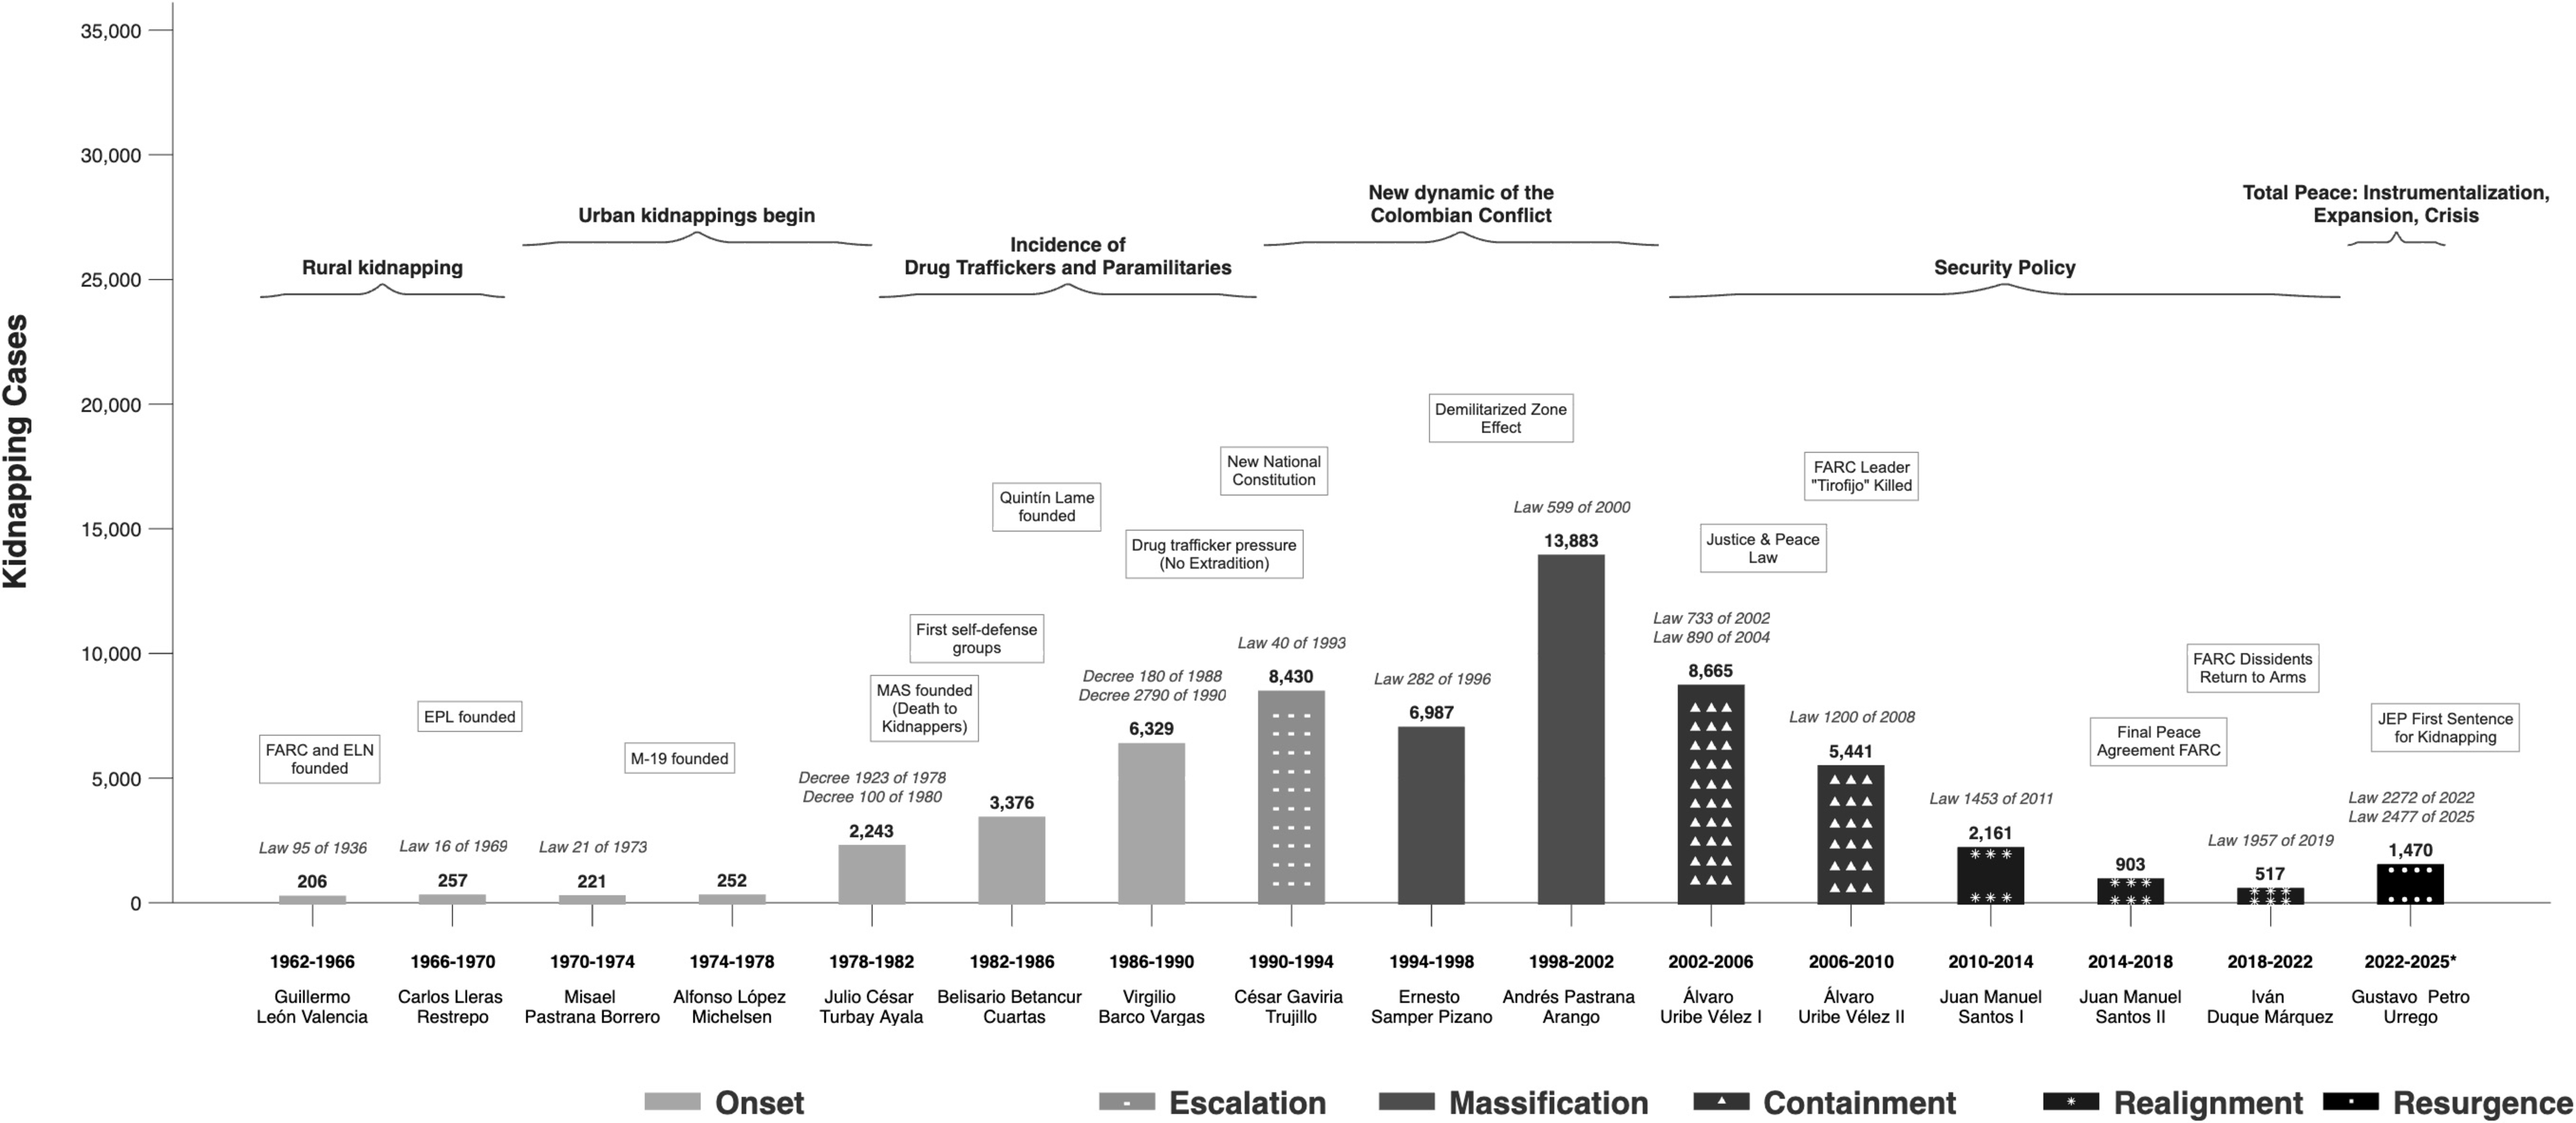
\includegraphics[width=\linewidth]{Fig_4.pdf}
\caption{Evolución del secuestro en Colombia: conflicto armado, política de seguridad y cambio institucional (1962--2025).}
\label{fig:evolucion-historica}
\figurenote{\textit{Nota:} La figura presenta el número total de secuestros por período presidencial en Colombia entre 1962 y 2025. El sombreado distingue las fases del conflicto armado, y las anotaciones destacan desarrollos relacionados con grupos armados, reformas legales y políticas de seguridad. \textit{Fuente:} Elaboración del autor con base en \citet{cnmh_datos} y \citet{pinto2004}.}
\end{figure}

A través de un modelo Logit Multinomial (MNL) y un modelo de riesgos proporcionales específicos por causa de \citet{Cox1972}, se cuantifica esta heterogeneidad a nivel organizacional. Ambos modelos se estiman sobre $n=1{,}125$ casos a nivel individual del Centro Nacional de Memoria Histórica, según \citet{cnmh_datos}, con especificación completa, pruebas de robustez y diagnósticos de selección muestral como se señala en el Apéndice B. La probabilidad marginal estática de mortalidad del MNL en cautiverio va de 0.002 para las FARC a 0.071 para la delincuencia común (DC). Las razones de hazard de pago relativas a las FARC alcanzan 4.28 para los paramilitares (PAR) y 1.71 para DC, mientras que el ELN es estadísticamente indistinguible del grupo de referencia. La probabilidad acumulada de rescate táctico al día 100 varía entre 0.27 y 0.33 según el tipo; después de 2011, el hazard de rescate se multiplica por 4.86 y el hazard de pago cae 49\%, consistente con el fortalecimiento de la capacidad disuasiva del GAULA, como se muestra en la Figura~\ref{fig:cox-a}. El perfil dinámico de mortalidad de Cox en la Figura~\ref{fig:cox-b} reproduce el mismo orden entre organizaciones, con magnitudes comparables (0.002 a 0.079). Estas estimaciones proveen el menú de tipos del mecanismo $\ThetaK=\{\text{DC},\text{PAR},\text{ELN},\text{FARC}\}$, ordenan la utilidad de reserva de la liberación $U^K_{\mathrm{rel}}(\theta)$ entre tipos, y anclan las intensidades efectivas específicas por tipo $\tilde\lambda_j(t\mid\theta_K)$ cuya separación empírica es la contraparte observacional de la hipótesis de separación en variación total del Lema~\ref{lem:hazard-separation}.

\begin{figure}[H]
\centering
\captionsetup[subfigure]{justification=centering,singlelinecheck=false}
\begin{subfigure}[t]{0.48\linewidth}
  \centering
  \parbox[t][\subfigheight][b]{\linewidth}{%
    \centering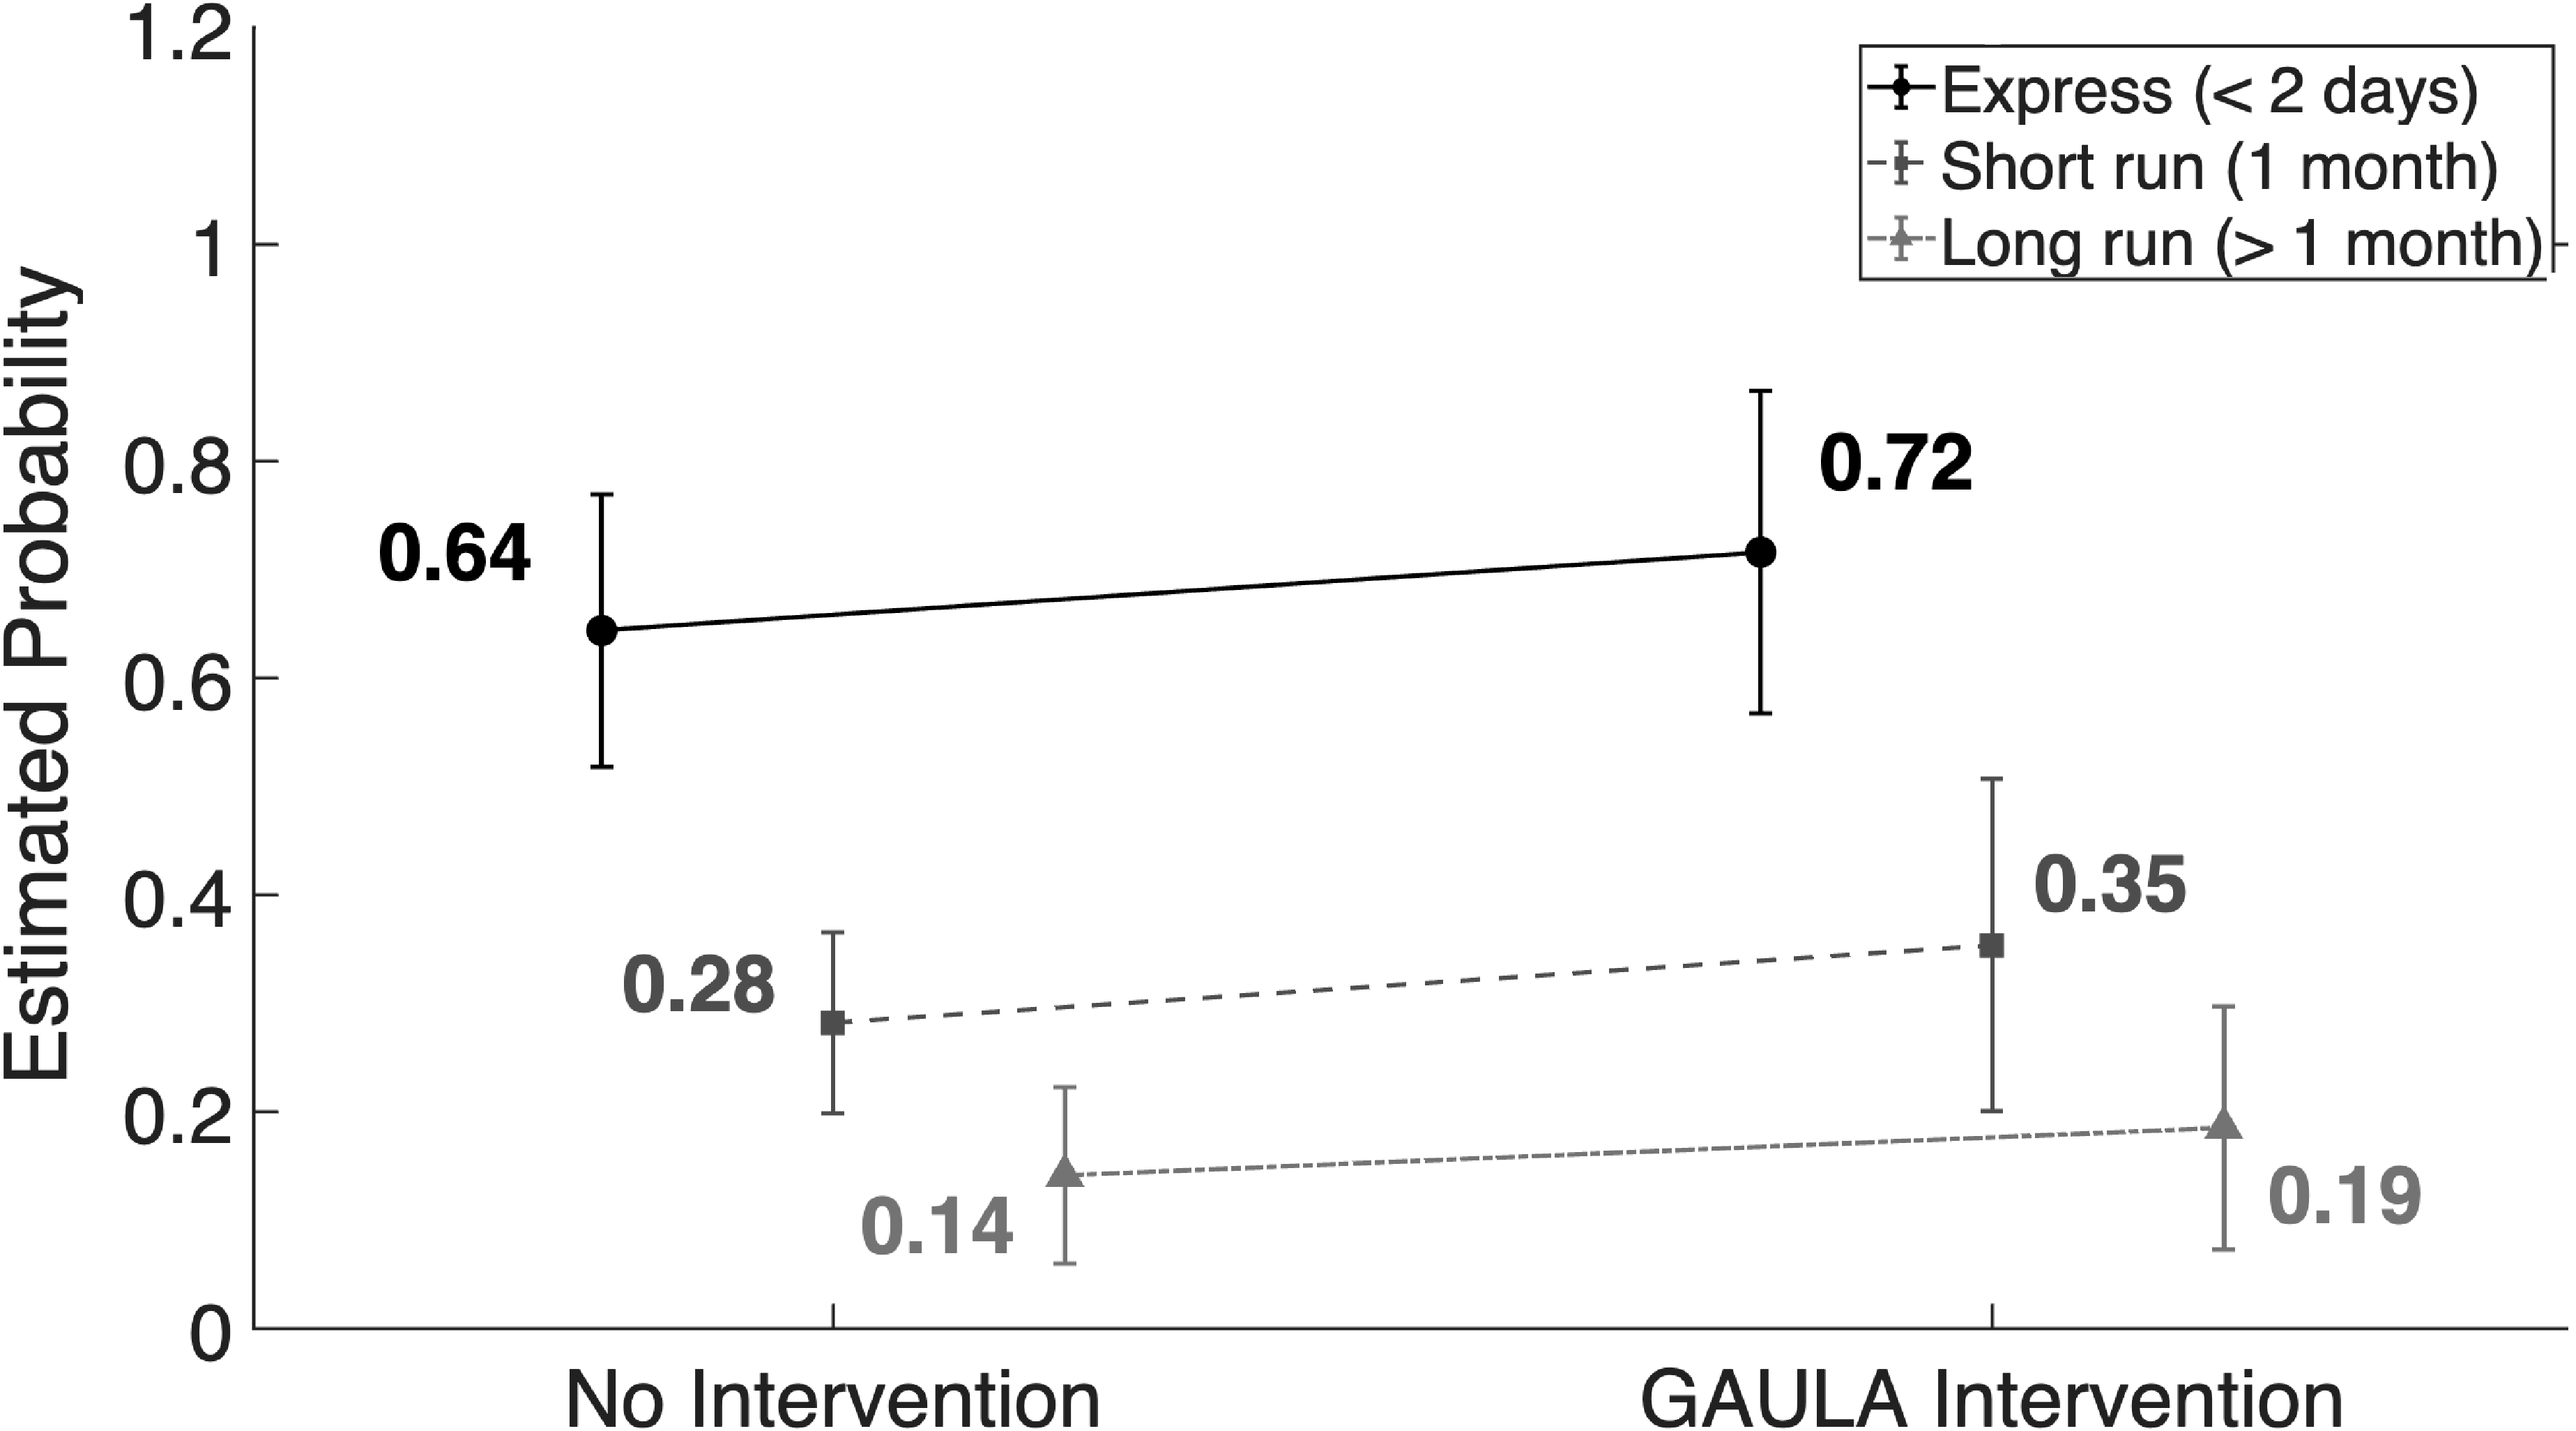
\includegraphics[width=\linewidth,height=\subfigheight,keepaspectratio]{Fig_9a.pdf}%
  }
  \caption{Rescate por intervención del GAULA y duración}
\end{subfigure}\hfill
\begin{subfigure}[t]{0.48\linewidth}
  \centering
  \parbox[t][\subfigheight][b]{\linewidth}{%
    \centering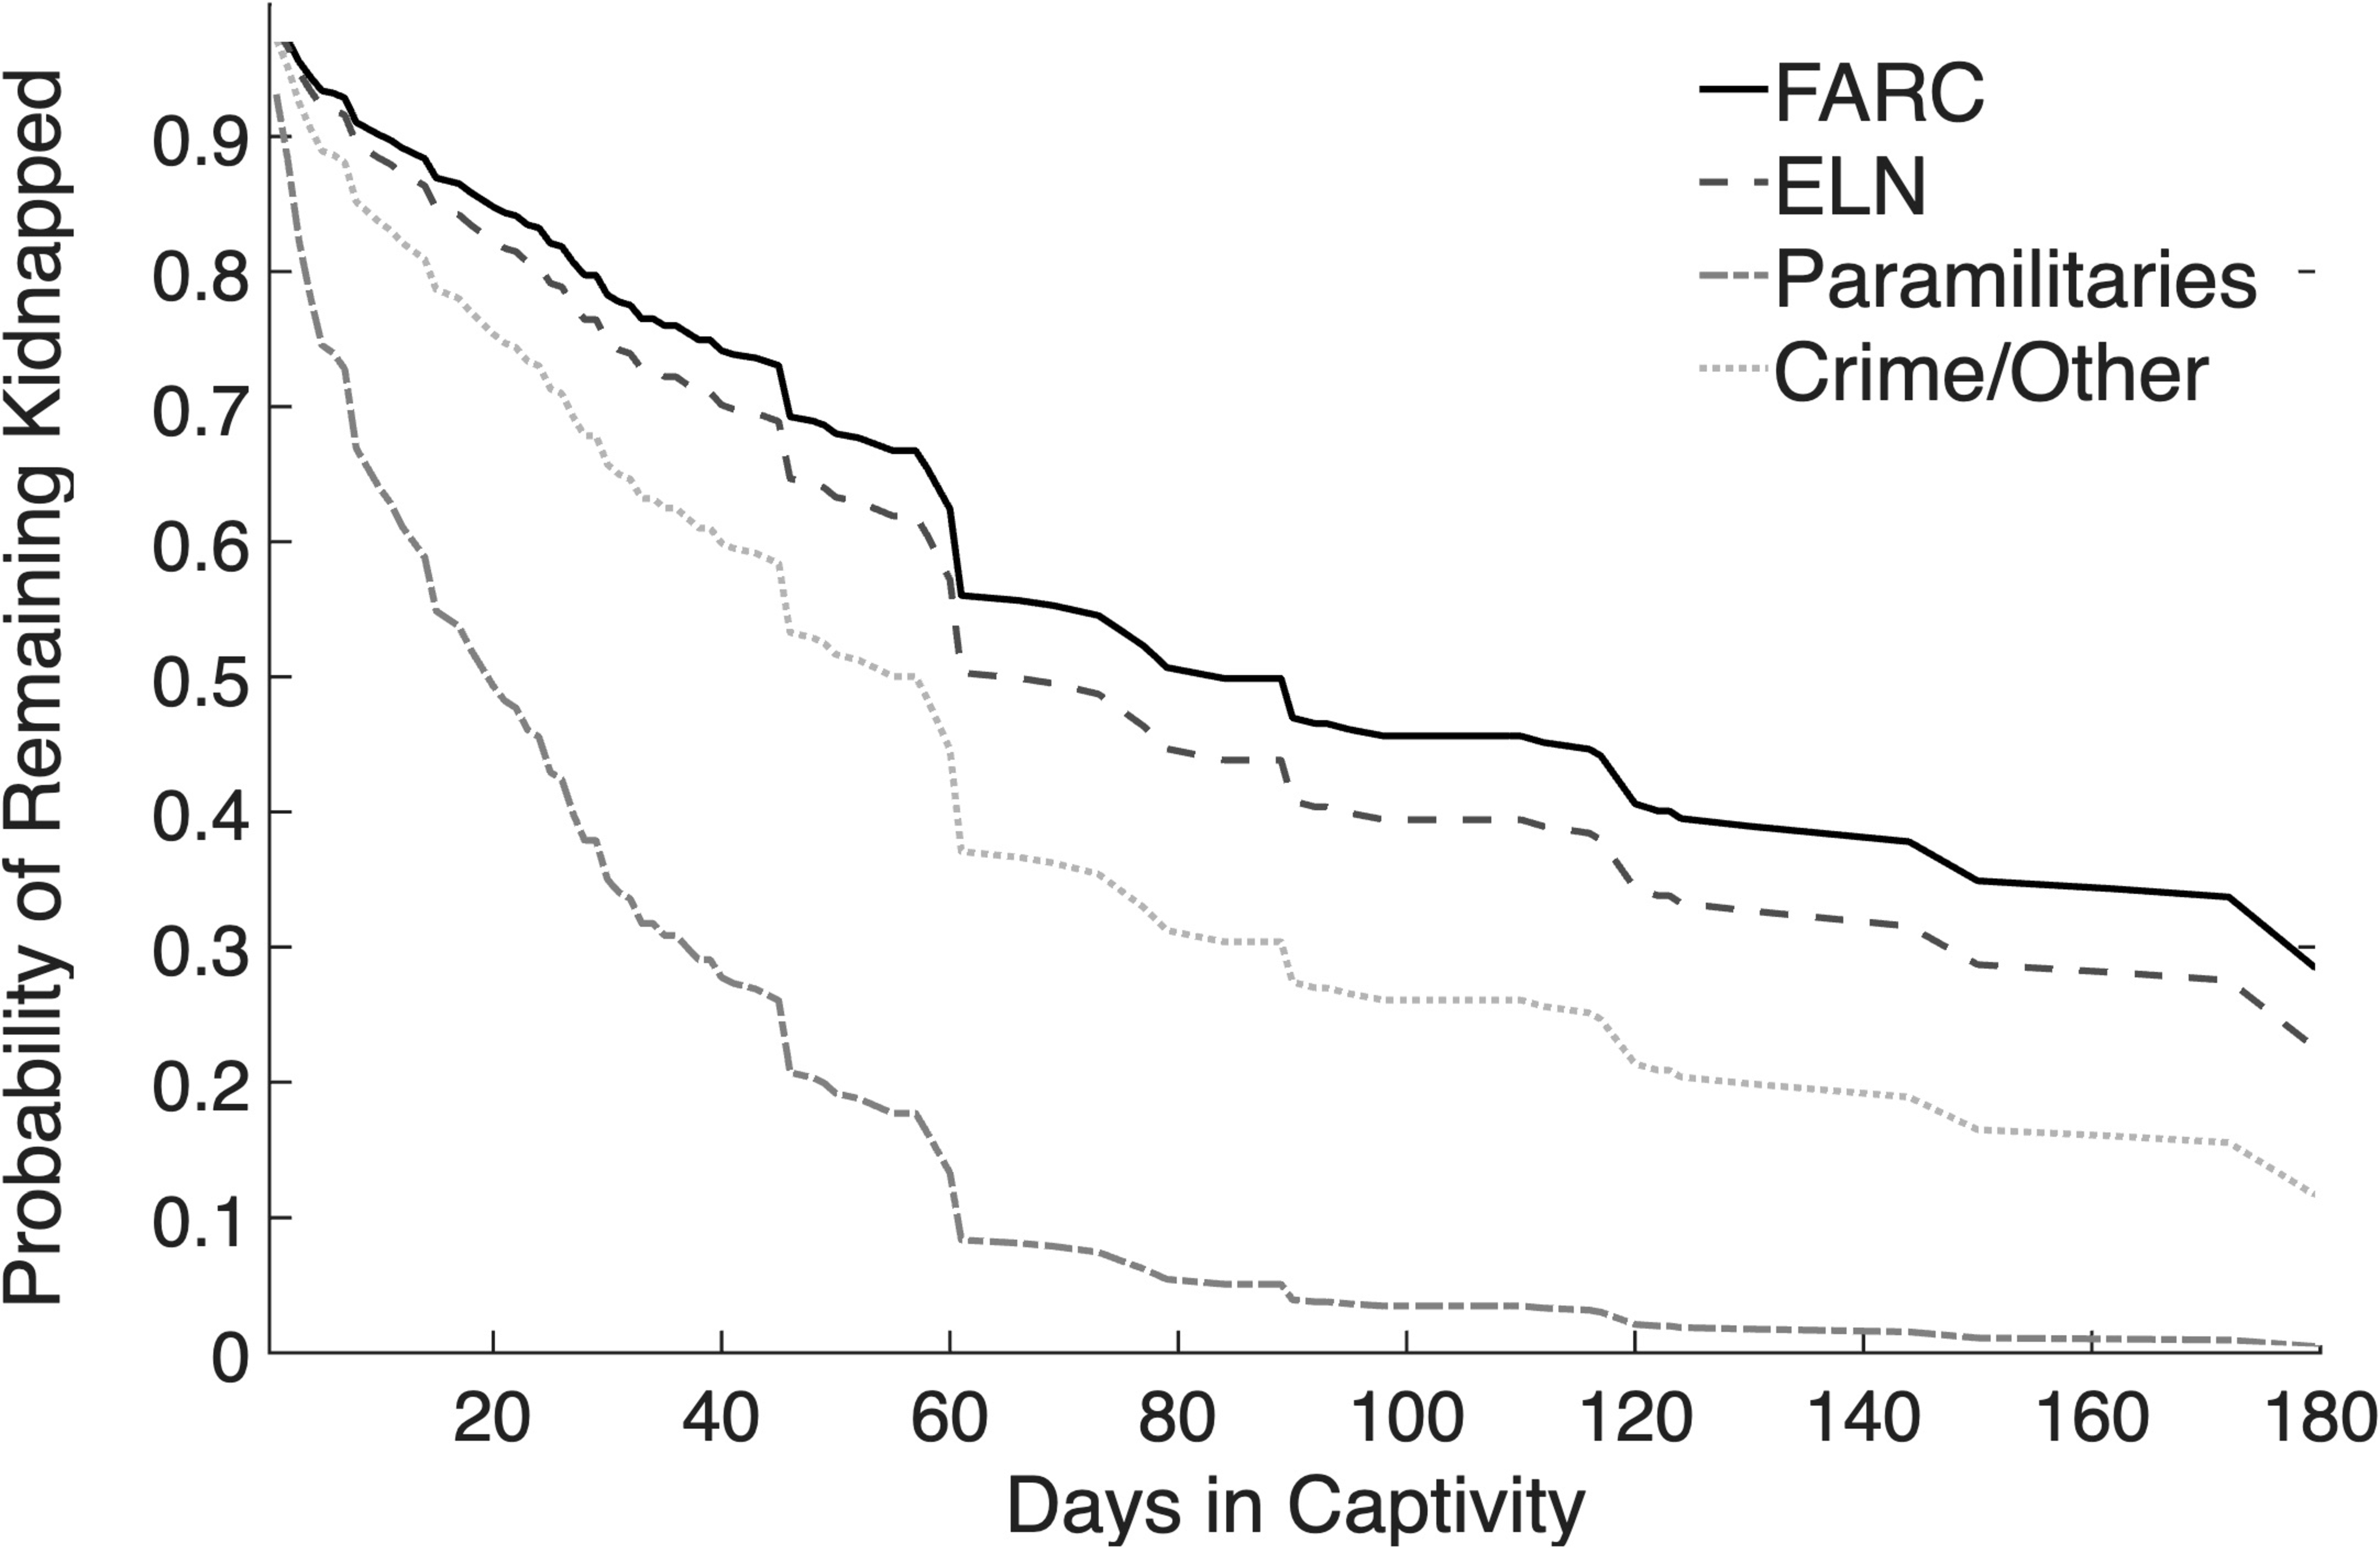
\includegraphics[width=\linewidth,height=\subfigheight,keepaspectratio]{Fig_9b.pdf}%
  }
  \caption{Supervivencia de la duración por perpetrador}
\end{subfigure}
\caption{Dinámica temporal del rescate y heterogeneidad en la duración del cautiverio.}
\label{fig:cox-a}
\figurenote{\textit{Nota:} El panel (a) reporta la probabilidad de Rescate según intervención del GAULA y categoría de duración. El panel (b) presenta las curvas de supervivencia de la duración del cautiverio por grupo perpetrador. \textit{Fuente:} Cálculos del autor con base en \citet{cnmh_datos}.}
\end{figure}

\begin{figure}[H]
\centering
\begin{subfigure}[t]{0.48\linewidth}
  \centering
  \panelgraphic{\subfigheight}{Fig_10a.pdf}
  \caption{Probabilidad acumulada de Rescate estatal}
\end{subfigure}\hfill
\begin{subfigure}[t]{0.48\linewidth}
  \centering
  \panelgraphic{\subfigheight}{Fig_10b.pdf}
  \caption{Mortalidad en cautiverio por grupo perpetrador}
\end{subfigure}
\caption{Probabilidad acumulada de rescate y mortalidad en cautiverio por grupo armado.}
\label{fig:cox-b}
\figurenote{\textit{Nota:} El panel (a) muestra la probabilidad acumulada de Rescate estatal por grupo armado, 1964--2025. El panel (b) reporta la probabilidad de Muerte en cautiverio por grupo perpetrador. \textit{Fuente:} Cálculos del autor con base en \citet{cnmh_datos}.}
\end{figure}

\subsection{De los estimadores a los insumos estructurales}\label{sec:pertinencia}

El MNL y el modelo de Cox conectan la evidencia microeconómica con la distribución inicial $\mu_0\in\Delta(\ThetaK)$ y los vectores de tecnología $\beta_{K,j}(\theta_K)$. El MNL provee la huella estática de cada tipo al relacionar perpetrador, víctima, contexto y tácticas con la distribución condicional de desenlaces; así, la creencia inicial y los pagos terminales se fijan con pesos observados. El modelo de Cox provee la dimensión dinámica: sus hazards específicos por causa se trasladan al mecanismo como tasas $\lambda_j(\theta_K,t)$ que gobiernan la señal diaria $\zeta_t$, actualizan el posterior $\mu_t$ y determinan la velocidad del aprendizaje. La separación empírica de esas tasas entre organizaciones es la base observacional del Lema~\ref{lem:hazard-separation} y del criterio de \citet{Kakutani1948}: si las trayectorias inducidas por los tipos generan leyes suficientemente distintas, el posterior puede concentrarse en el tipo verdadero. En conjunto, este bloque microeconométrico convierte los datos a nivel de caso en priors, costos, hazards y restricciones directamente utilizables por el mecanismo dinámico. El protocolo explícito de traducción entre estimadores y parámetros estructurales se detalla al comienzo de la Sección~\ref{sec:calibracion}.

\section{Calibración del mecanismo y simulaciones}\label{sec:calibracion}
\normalfont\normalsize
Esta sección calibra el mecanismo especializado de la Sección~\ref{sec:application} en cuatro episodios simulados de horizonte finito, manteniendo fija la arquitectura general de la Sección~\ref{sec:model}. El ejercicio combina priors y diagnósticos microeconométricos para estudiar cuatro objetos: la evolución de las creencias $\mu_t(\theta)$, las señales observadas por el Estado, la respuesta de los instrumentos $(\alpha_t,\gamma_t)$, y el cumplimiento de las restricciones IR e IC. El \emph{Escenario~I} corresponde a DC, con $\theta_K^\ast=\mathrm{DC}$, Estado laxo, familia de alta riqueza, víctima privada, y localización Metrópoli; el \emph{Escenario~II} corresponde a PAR, con $\theta_K^\ast=\mathrm{PAR}$, Estado estricto, familia de riqueza estándar, víctima pública, y localización Caribe; el \emph{Escenario~III} corresponde a ELN, con $\theta_K^\ast=\mathrm{ELN}$, Estado estricto, familia de alta riqueza, víctima privada, y localización Oriente-Selva; y el \emph{Escenario~IV} corresponde a FARC, con $\theta_K^\ast=\mathrm{FARC}$, Estado laxo, familia de alta riqueza, víctima pública, y localización Pacífico / Zona Roja. Ambos se simulan sobre un horizonte fijo $\bar{T}=150$ períodos, y la política óptima se calcula a partir de la minimización del costo social del Estado. En el orden $(\mathrm{DC},\mathrm{PAR},\mathrm{ELN},\mathrm{FARC})$, los priors iniciales son $\mu_0^{\mathrm{DC}}=(0.35,0.35,0.15,0.15)$, $\mu_0^{\mathrm{PAR}}=(0.15,0.15,0.25,0.45)$, $\mu_0^{\mathrm{ELN}}=(0.05,0.35,0.25,0.35)$, y $\mu_0^{\mathrm{FARC}}=(0.35,0.35,0.15,0.15)$. En las figuras, la barra gris marca el tiempo de parada realizado $\tau$; la trayectoria posterior a esa barra es una extensión contrafactual bajo un estado absorbente, siguiendo la ley del mecanismo condicionada a la no absorción, que ilustra la dinámica de aprendizaje e identificación independientemente del momento de cierre, sin constituir una trayectoria real de episodio.

A diferencia de una política puramente miope que omite el término $-\psi_H\Delta H_t$, la regla calibrada en este modelo internaliza el subsidio informacional del Estado, lo que le permite reasignar estratégicamente los instrumentos $(\alpha_t,\gamma_t)$ hacia zonas de la grilla que maximizan la separación de las verosimilitudes de los tipos rivales. De este modo, los ejercicios numéricos para los casos DC, PAR, ELN y FARC permiten ilustrar tres implicaciones operativas fundamentales de la teoría: en primer lugar, la concentración de la creencia posterior en un horizonte finito en la dirección que predice el Teorema~\ref{thm:posterior-consistency}; en segundo lugar, la actualización bayesiana con soporte completo a lo largo de las trayectorias que habilita el MDG; y, en tercer lugar, el cumplimiento ex-post de las restricciones $IC^K$, $IR^K$ e $IR^F$ conforme a la lógica de implementabilidad descrita en el Teorema~\ref{thm:ebp-implementabilidad}. Conviene subrayar que estas simulaciones ilustran el aprendizaje a horizonte finito y no pretenden demostrar la identificación asintótica sobre $\mathcal{T}$, la cual se mantiene estrictamente como un resultado teórico límite.


\begin{figure}[H]
\centering
\begin{subfigure}[t]{0.48\linewidth}
  \centering
  \panelgraphic{\calbeliefheight}{Fig_11a.pdf}
  \caption{Escenario I: DC}
\end{subfigure}\hfill
\begin{subfigure}[t]{0.48\linewidth}
  \centering
  \panelgraphic{\calbeliefheight}{Fig_11b.pdf}
  \caption{Escenario II: PAR}
\end{subfigure}

\medskip
\begin{subfigure}[t]{0.48\linewidth}
  \centering
  \panelgraphic{\calbeliefheight}{Fig_11c.pdf}
  \caption{Escenario III: ELN}
\end{subfigure}\hfill
\begin{subfigure}[t]{0.48\linewidth}
  \centering
  \panelgraphic{\calbeliefheight}{Fig_11d.pdf}
  \caption{Escenario IV: FARC}
\end{subfigure}
\caption{Creencias bayesianas de cada tipo $\mu_\tau(\theta)$ en los diferentes escenarios.}
\label{fig:cal-eln-par-mu}
\figurenote{\textit{Nota:} El panel (a) corresponde al Escenario~I: $\theta_K^\ast=\mathrm{DC}$, $\theta_S$ laxo, $\theta_F$ de alta riqueza, $\theta_V$ privado, y $z$ Metrópoli. El panel (b) corresponde al Escenario~II: $\theta_K^\ast=\mathrm{PAR}$, $\theta_S$ estricto, $\theta_F$ de riqueza estándar, $\theta_V$ público, y $z$ Caribe. El panel (c) corresponde al Escenario~III: $\theta_K^\ast=\mathrm{ELN}$, $\theta_S$ estricto, $\theta_F$ de alta riqueza, $\theta_V$ privado, y $z$ Oriente-Selva. El panel (d) corresponde al Escenario~IV: $\theta_K^\ast=\mathrm{FARC}$, $\theta_S$ laxo, $\theta_F$ de alta riqueza, $\theta_V$ público, y $z$ Pacífico / Zona Roja. La banda gris marca $\tau^{\mathrm{hyp}}$, el primer período en el que el resultado del mecanismo difiere de la continuación.}
\end{figure}
\vspace{-8pt}
El posterior del tipo verdadero permite evaluar la capacidad del mecanismo para separar tipos a partir de la secuencia de señales. Como se reporta en la Figura~\ref{fig:cal-eln-par-mu}, la masa posterior se desplaza gradualmente hacia el tipo verdadero en los cuatro escenarios, alcanzando $\mu_{150}(\theta_K^\ast)\approx 1{,}000$; esto implica que el mecanismo acumula identificación bajo diferentes niveles de riqueza, regiones y visibilidad. En el Escenario~I y el Escenario~IV, la concentración posterior es rápida. En el Escenario~II y el Escenario~III, las trayectorias son menos monótonas en la fase inicial, lo que refleja señales tempranas compatibles con tipos alternativos antes de que la masa se desplace definitivamente hacia el verdadero captor. Las barras grises marcan el tiempo de parada realizado; la extensión contrafactual subsiguiente muestra que la velocidad de aprendizaje y el momento de absorción son objetos distintos del modelo. En conjunto, la figura ilustra el comportamiento a horizonte finito: la masa posterior se desplaza hacia el tipo verdadero a medida que las señales acumulan separación, en la dirección predicha por el Teorema~\ref{thm:posterior-consistency} bajo $\mathcal{T}$, sin constituir evidencia directa del resultado asintótico; la velocidad de convergencia depende del entorno institucional, territorial, y de visibilidad del caso.

\begin{figure}[H]
\centering
\begin{subfigure}[t]{0.48\linewidth}
  \centering
  \panelgraphic{\calseriesheight}{Fig_12a.pdf}
  \caption{Escenario I: DC}
\end{subfigure}\hfill
\begin{subfigure}[t]{0.48\linewidth}
  \centering
  \panelgraphic{\calseriesheight}{Fig_12b.pdf}
  \caption{Escenario II: PAR}
\end{subfigure}

\medskip
\begin{subfigure}[t]{0.48\linewidth}
  \centering
  \panelgraphic{\calseriesheight}{Fig_12c.pdf}
  \caption{Escenario III: ELN}
\end{subfigure}\hfill
\begin{subfigure}[t]{0.48\linewidth}
  \centering
  \panelgraphic{\calseriesheight}{Fig_12d.pdf}
  \caption{Escenario IV: FARC}
\end{subfigure}
\caption{Presión operativa $\gamma_t^\ast$ y punto de referencia $\gamma^R$ frente a $\tau$.}
\label{fig:cal-eln-par-gamma}
\figurenote{\textit{Nota:} El panel (a) muestra la trayectoria de presión operativa en el Escenario~I (DC). El panel (b) muestra la trayectoria equivalente en el Escenario~II (PAR). El panel (c) muestra el Escenario~III (ELN). El panel (d) muestra el Escenario~IV (FARC). La línea punteada corresponde al punto de referencia de Rescate $\gamma^R$. La banda gris marca $\tau^{\mathrm{hyp}}$.}
\end{figure}
La presión operativa óptima permite evaluar cómo ajusta el Estado la intensidad de la intervención a medida que aprende sobre el tipo del captor. La Figura~\ref{fig:cal-eln-par-gamma} compara la trayectoria de $\gamma_t^\ast$ con el punto de referencia de Rescate $\gamma^R$, que toma el valor $\gamma^R=0{,}23$ en DC, $\gamma^R=0{,}37$ en PAR, $\gamma^R=0{,}50$ en ELN y $\gamma^R=0{,}64$ en FARC. En el Escenario~I (DC), $\gamma_t^\ast$ se ubica en promedio alrededor de $\bar\gamma^\ast\approx 0{,}564$. En el Escenario~II (PAR), la presión alcanza $\bar\gamma^\ast\approx 0{,}662$. En el Escenario~III (ELN), la presión promedio es $\bar\gamma^\ast\approx 0{,}663$, y en el Escenario~IV (FARC) alcanza $\bar\gamma^\ast\approx 0{,}715$. En todos los casos, $\gamma_t^\ast$ no replica mecánicamente ni la rama de Rescate ni la de Negociación: el control dual combina la explotación del instrumento y la información esperada, de modo que la serie fluctúa entre puntos de referencia según el riesgo material del episodio y el valor de separar tipos.

La interdicción financiera óptima resume la intensidad con la que el Estado restringe la capacidad de pago y la coordinación económica durante el episodio. La Figura~\ref{fig:cal-eln-par-alpha} compara la trayectoria de $\alpha_t^\ast$ con el punto de referencia de Rescate $\alpha^R$, que toma el valor $\alpha^R=0{,}18$ en DC, $\alpha^R=0{,}31$ en PAR, $\alpha^R=0{,}45$ en ELN y $\alpha^R=0{,}59$ en FARC. En el Escenario~I (DC), $\bar\alpha^\ast\approx 0{,}896$. En el Escenario~II (PAR), $\bar\alpha^\ast\approx 0{,}730$. En el Escenario~III (ELN), $\bar\alpha^\ast\approx 0{,}737$, y en el Escenario~IV (FARC), $\bar\alpha^\ast\approx 0{,}755$. Así, $\alpha_t^\ast$ no replica mecánicamente una rama pura: se mueve entre los puntos de referencia de Rescate y Negociación según la información acumulada, la capacidad de pago de la familia, y el valor de inducir separación entre tipos.

La precisión posterior, definida como $\iota_t=\max_{\theta\in\ThetaK}\mu_t(\theta)$, permite observar cómo cambia la presión operativa cuando el Estado gana confianza sobre la identidad del tipo verdadero. La Figura~\ref{fig:cal-eln-par-iota-gamma} reordena la simulación sobre el plano $(\iota_t,\gamma_t^\ast)$; las flechas indican el avance de $\tau$ y evitan interpretar las observaciones como una interpolación lineal. La trayectoria se concentra en zonas de alta presión y precisión creciente, reflejando aprendizaje sin colapso inmediato hacia una única señal dominante, y mostrando las diferentes dinámicas entre casos.
\vspace{-4pt}
\begin{figure}[H]
\centering
\begin{subfigure}[t]{0.48\linewidth}
  \centering
  \panelgraphic{\calseriesheight}{Fig_13a.pdf}
  \caption{Escenario I: DC}
\end{subfigure}\hfill
\begin{subfigure}[t]{0.48\linewidth}
  \centering
  \panelgraphic{\calseriesheight}{Fig_13b.pdf}
  \caption{Escenario II: PAR}
\end{subfigure}

\medskip
\begin{subfigure}[t]{0.48\linewidth}
  \centering
  \panelgraphic{\calseriesheight}{Fig_13c.pdf}
  \caption{Escenario III: ELN}
\end{subfigure}\hfill
\begin{subfigure}[t]{0.48\linewidth}
  \centering
  \panelgraphic{\calseriesheight}{Fig_13d.pdf}
  \caption{Escenario IV: FARC}
\end{subfigure}
\caption{Interdicción financiera $\alpha_t^\ast$ y punto de referencia $\alpha^R$ frente a $\tau$.}
\label{fig:cal-eln-par-alpha}
\figurenote{\textit{Note:} El panel (a) presenta la interdicción financiera óptima en el Escenario~I (DC). El panel (b) presenta el Escenario~II (PAR). El panel (c) presenta el Escenario~III (ELN). El panel (d) presenta el Escenario~IV (FARC). La línea punteada corresponde al punto de referencia de Rescate $\alpha^R$. La banda gris marca $\tau^{\mathrm{hyp}}$.}
\end{figure}
\vspace{-6pt}
La interdicción financiera frente a la precisión posterior permite evaluar si el aprendizaje reduce o refuerza la necesidad de restringir la capacidad de pago. Como se reporta en la Figura~\ref{fig:cal-eln-par-iota-alpha}, $\alpha_t^\ast$ permanece alto mientras $\iota_t$ aumenta en todos los escenarios, lo que indica que identificar el tipo verdadero no elimina el valor de mantener la interdicción preventiva. Este patrón es consistente con entornos donde la interdicción financiera conserva relevancia como instrumento de control, contención de pagos, e inducción de separación entre tipos.
\vspace{-4pt}
\begin{figure}[H]
\centering
\begin{subfigure}[t]{0.48\linewidth}
  \centering
  \panelgraphic{\calfigheight}{Fig_14a.pdf}
  \caption{Escenario I: DC}
\end{subfigure}\hfill
\begin{subfigure}[t]{0.48\linewidth}
  \centering
  \panelgraphic{\calfigheight}{Fig_14b.pdf}
  \caption{Escenario II: PAR}
\end{subfigure}

\medskip
\begin{subfigure}[t]{0.48\linewidth}
  \centering
  \panelgraphic{\calfigheight}{Fig_14c.pdf}
  \caption{Escenario III: ELN}
\end{subfigure}\hfill
\begin{subfigure}[t]{0.48\linewidth}
  \centering
  \panelgraphic{\calfigheight}{Fig_14d.pdf}
  \caption{Escenario IV: FARC}
\end{subfigure}
\caption{Trayectoria $(\iota_t,\gamma_t^\ast)$ con flechas que indican el avance temporal.}
\label{fig:cal-eln-par-iota-gamma}
\figurenote{\textit{Nota:} El panel (a) corresponde al Escenario~I (DC), el panel (b) al Escenario~II (PAR), el panel (c) al Escenario~III (ELN), y el panel (d) al Escenario~IV (FARC). Cada trayectoria muestra 20 flechas indicadoras; el círculo identifica el punto final, $\tau=150$.}
\end{figure}
\vspace{-6pt}
El diagnóstico de restricciones confirma que la factibilidad estratégica del mecanismo se preserva en todos los escenarios. Como muestra la Figura~\ref{fig:cal-eln-par-iric}, la restricción de incentivos del captor ($\mathrm{IC}^K$), la restricción de participación del captor ($\mathrm{IR}^K$), y la restricción de participación de la familia ($\mathrm{IR}^F$) se satisfacen en los 150 ciclos simulados en los cuatro escenarios. La verificación es \emph{a posteriori} respecto al tipo verdadero $\theta_K^\ast$: los instrumentos óptimos $(a_S^\ast,\alpha_t^\ast,\gamma_t^\ast)$ se evalúan directamente sobre las utilidades del tipo verdadero, sin ponderar por la creencia $\mu_t$. El mecanismo es por lo tanto factible en un sentido ex-post: dado $\theta_K^\ast$, la política óptima satisface la compatibilidad de incentivos y la participación sin abandonar el componente informacional.
\vspace{-4pt}
\begin{figure}[H]
\centering
\begin{subfigure}[t]{0.48\linewidth}
  \centering
  \panelgraphic{\calfigheight}{Fig_15a.pdf}
  \caption{Escenario I: DC}
\end{subfigure}\hfill
\begin{subfigure}[t]{0.48\linewidth}
  \centering
  \panelgraphic{\calfigheight}{Fig_15b.pdf}
  \caption{Escenario II: PAR}
\end{subfigure}

\medskip
\begin{subfigure}[t]{0.48\linewidth}
  \centering
  \panelgraphic{\calfigheight}{Fig_15c.pdf}
  \caption{Escenario III: ELN}
\end{subfigure}\hfill
\begin{subfigure}[t]{0.48\linewidth}
  \centering
  \panelgraphic{\calfigheight}{Fig_15d.pdf}
  \caption{Escenario IV: FARC}
\end{subfigure}
\caption{Trayectoria $(\iota_t,\alpha_t^\ast)$ con flechas que indican el avance temporal.}
\label{fig:cal-eln-par-iota-alpha}
\figurenote{\textit{Note:} El panel (a) corresponde al Escenario~I (DC), el panel (b) al Escenario~II (PAR), el panel (c) al Escenario~III (ELN), y el panel (d) al Escenario~IV (FARC). Cada trayectoria muestra 20 flechas indicadoras; el círculo identifica el punto final, $\tau=150$.}
\end{figure}
\clearpage
\begin{figure}[H]
\centering
\begin{subfigure}[t]{0.48\linewidth}
  \centering
  \panelgraphic{\calfigheight}{Fig_16a.pdf}
  \caption{Escenario I: DC}
\end{subfigure}\hfill
\begin{subfigure}[t]{0.48\linewidth}
  \centering
  \panelgraphic{\calfigheight}{Fig_16b.pdf}
  \caption{Escenario II: PAR}
\end{subfigure}

\medskip
\begin{subfigure}[t]{0.48\linewidth}
  \centering
  \panelgraphic{\calfigheight}{Fig_16c.pdf}
  \caption{Escenario III: ELN}
\end{subfigure}\hfill
\begin{subfigure}[t]{0.48\linewidth}
  \centering
  \panelgraphic{\calfigheight}{Fig_16d.pdf}
  \caption{Escenario IV: FARC}
\end{subfigure}
\caption{Frecuencia de cumplimiento de $\mathrm{IC}^K$, $\mathrm{IR}^K$, e $\mathrm{IR}^F$ (\% de ciclos).}
\label{fig:cal-eln-par-iric}
\figurenote{\textit{Nota:} El panel (a) resume el cumplimiento en el Escenario~I (DC), el panel (b) en el Escenario~II (PAR), el panel (c) en el Escenario~III (ELN), y el panel (d) en el Escenario~IV (FARC). Los porcentajes se calculan sobre los ciclos simulados de cada escenario.}
\end{figure}
\vspace{-6pt}
La ganancia informacional esperada $\Delta H_t$ cuantifica la reducción anticipada de entropía inducida por los instrumentos del Estado, en el sentido de la adquisición dinámica óptima de información de \citet{Zhong2022}. Ese subsidio informacional se concentra al inicio de la simulación, como se ilustra en la Figura~\ref{fig:cal-eln-par-dh}: en DC alcanza su máximo en $\tau=10$ con $\Delta H_{10}\approx 0{,}043$, y en PAR en $\tau=6$ con $\Delta H_6\approx 0{,}035$. A medida que $\Delta H_t$ converge a cero, las observaciones adicionales dejan de reducir la incertidumbre posterior y la decisión óptima pasa a estar gobernada por las pérdidas materiales y una creencia ya concentrada en el tipo verdadero.
\vspace{-4pt}
\begin{figure}[H]
\centering
\begin{subfigure}[t]{0.48\linewidth}
  \centering
  \panelgraphic{\calfigheight}{Fig_17a.pdf}
  \caption{Escenario I: DC}
\end{subfigure}\hfill
\begin{subfigure}[t]{0.48\linewidth}
  \centering
  \panelgraphic{\calfigheight}{Fig_17b.pdf}
  \caption{Escenario II: PAR}
\end{subfigure}

\medskip
\begin{subfigure}[t]{0.48\linewidth}
  \centering
  \panelgraphic{\calfigheight}{Fig_17c.pdf}
  \caption{Escenario III: ELN}
\end{subfigure}\hfill
\begin{subfigure}[t]{0.48\linewidth}
  \centering
  \panelgraphic{\calfigheight}{Fig_17d.pdf}
  \caption{Escenario IV: FARC}
\end{subfigure}
\caption{Ganancia informacional esperada $\Delta H_t$ frente a $\tau$.}
\label{fig:cal-eln-par-dh}
\figurenote{\textit{Nota:} El panel (a) corresponde al Escenario~I (DC), el panel (b) al Escenario~II (PAR), el panel (c) al Escenario~III (ELN), y el panel (d) al Escenario~IV (FARC). La serie reporta la reducción esperada de entropía en cada ciclo simulado.}
\end{figure}
\vspace{-6pt}
En todos los escenarios y para todos los tipos, $\kappa_h(\theta_K^\ast,t)>0$ en el 100\,\% de los ciclos simulados, como se muestra en la Figura~\ref{fig:cal-eln-par-kh}. Por la relación $\operatorname{sgn}(\partial\,\mathbb{E}[\tau\mid\theta_K]/\partial\gamma_t^\ast)=-\operatorname{sgn}(\kappa_h)$, esto implica $\partial\,\mathbb{E}[\tau\mid\theta_K]/\partial\gamma_t^\ast<0$: una mayor presión operativa \emph{reduce} la duración esperada del cautiverio sin excepción. El mecanismo no enfrenta un trade-off entre explotar el instrumento y aprender: la presión operativa acorta el cautiverio y, al modificar los hazards de cierre, genera simultáneamente señales que separan las verosimilitudes de los tipos rivales y aceleran la convergencia posterior.
\vspace{-4pt}
\begin{figure}[H]
\centering
\begin{subfigure}[t]{0.48\linewidth}
  \centering
  \panelgraphic{\calseriesheight}{Fig_18a.pdf}
  \caption{Escenario I: DC}
\end{subfigure}\hfill
\begin{subfigure}[t]{0.48\linewidth}
  \centering
  \panelgraphic{\calseriesheight}{Fig_18b.pdf}
  \caption{Escenario II: PAR}
\end{subfigure}

\medskip
\begin{subfigure}[t]{0.48\linewidth}
  \centering
  \panelgraphic{\calseriesheight}{Fig_18c.pdf}
  \caption{Escenario III: ELN}
\end{subfigure}\hfill
\begin{subfigure}[t]{0.48\linewidth}
  \centering
  \panelgraphic{\calseriesheight}{Fig_18d.pdf}
  \caption{Escenario IV: FARC}
\end{subfigure}
\caption{Sensibilidad neta $\kappa_h(\theta_K^\ast,t)$ de la duración esperada del cautiverio respecto a $\gamma_t^\ast$.}
\label{fig:cal-eln-par-kh}
\figurenote{\textit{Nota:} Cada panel traza $\kappa_h(\theta_K^\ast,t)$ para el tipo verdadero del escenario. Un valor constante de $+1$ implica $-\operatorname{sgn}(\kappa_h)=-1$ en el 100\,\% de los ciclos, es decir, $\partial\,\mathbb{E}[\tau\mid\theta_K]/\partial\gamma_t^\ast<0$; la línea punteada horizontal marca el cero de referencia.}
\end{figure}
\vspace{-6pt}
Los desenlaces terminales hipotéticos difieren entre escenarios: \emph{Pago} en DC ($\tau^{\mathrm{hyp}}=35$), \emph{Rescate} en PAR ($\tau^{\mathrm{hyp}}=105$), \emph{Liberación} en ELN ($\tau^{\mathrm{hyp}}=75$), y \emph{Rescate} en FARC ($\tau^{\mathrm{hyp}}=20$). En todos los casos el posterior parte de su prior inicial y converge a $\mu_{150}(\theta^\ast)\approx 1{,}000$, con $\bar\alpha^\ast$ y $\bar\gamma^\ast$ por encima de 0{,}56 en todos los escenarios. Estos resultados se resumen en la Tabla~\ref{tab:calibracion-resumen}.

\begin{table}[htbp]
\centering
\caption{Resumen de la calibración dinámica por escenario}
\label{tab:calibracion-resumen}
\small
\begin{tabular}{lrrrrrl}
\toprule
$\theta_K^\ast$ & $\mu_0(\theta^\ast)$ & $\mu_{\tau_{\max}}(\theta^\ast)$ & $\bar{\alpha}^\ast$ & $\bar{\gamma}^\ast$ & $\tau^{\mathrm{hyp}}$ & $m_{\tau^{\mathrm{hyp}}}$ \\
\midrule
DC & 0.350 & 1.000 & 0.896 & 0.564 & 35 & Pago \\
PAR & 0.150 & 1.000 & 0.730 & 0.662 & 105 & Rescate \\
ELN & 0.250 & 1.000 & 0.737 & 0.663 & 75 & Liberación \\
FARC & 0.150 & 1.000 & 0.755 & 0.715 & 20 & Rescate \\
\bottomrule
\end{tabular}
\end{table}En conjunto, el contraste ELN--PAR muestra que el mismo mecanismo bayesiano genera trayectorias de aprendizaje, intensidades de instrumentos, y tasas de viabilidad de restricciones distintas cuando, conjuntamente, cambian el tipo verdadero del captor y los márgenes institucional, familiar, de víctima, y geográfico descritos en el protocolo. Las simulaciones no sustituyen al Teorema~\ref{thm:posterior-consistency}, que requiere separación recurrente en el evento $\mathcal{T}$; ilustran que, con priors y hazards calibrados a la evidencia colombiana, el subsidio entrópico desplaza la política lejos de regímenes puramente miopes y acelera o disciplina la concentración posterior en horizontes finitos, en la dirección predicha por el resultado de identificación.

\section{Discusión y conclusiones}\label{sec:conclusiones}

Este artículo desarrolla un mecanismo indirecto dinámico para entornos en los que las acciones de equilibrio se agrupan y los tipos no se elicitan mediante reportes libres. Respecto a la reducción clásica vía el Principio de Revelación, la contribución es construir el objeto indirecto operativo: instrumentos públicos, ruido de implementación endógeno y aprendizaje bayesiano sobre señales generadas por acciones.

A nivel teórico, el núcleo MDG provee la materialización con soporte completo de las intenciones latentes sin un temblor exógeno, manteniendo la regla de Bayes bien definida fuera de la senda. El Teorema de Identificación de Tipos muestra que la separación recurrente en variación total de las leyes de observación condicionales al tipo implica la singularidad mutua de las medidas de trayectoria y la concentración posterior casi segura en el tipo verdadero en el evento de interacción prolongada $\mathcal{T}$. El Teorema de Implementabilidad Condicional complementa la identificación al garantizar un EBP que satisface la compatibilidad de incentivos y la racionalidad individual siempre que el conjunto factible permanezca no vacío. El resultado asintótico es deliberadamente preciso: clarifica el límite informacional de la arquitectura; el comportamiento en horizonte finito es un objeto distinto y aplicado.

A nivel aplicado, el secuestro extorsivo en Colombia mapea el espacio de tipos abstracto a tecnologías criminales estimadas. La evidencia de riesgos competitivos y multinomial disciplina los hazards y los priors; las simulaciones ELN--PAR muestran que la regla calibrada de control dual acelera la concentración posterior, sostiene instrumentos altos pero disciplinados y preserva la factibilidad IR/IC, en la dirección predicha por los teoremas sin sustituirlos.

Dos extensiones son naturales. La primera es una cota de identificación en horizonte finito que traduzca la separación en variación total en tasas explícitas de concentración posterior bajo parada endógena. La segunda es la identificación concurrente con múltiples agentes cuando varias partes con información privada interactúan bajo una historia pública compartida. Ambas trasladarían el marco más allá del cribado adversarial a otros mercados con implementación ruidosa y agrupamiento observacional.


\section*{Declaración sobre el uso de Inteligencia Artificial Generativa}

En la preparación de este manuscrito, el autor utilizó herramientas de inteligencia artificial generativa, específicamente \emph{Cursor} y \emph{Antigravity}, para asistir en las siguientes tareas: revisión de literatura y edición de texto; programación en Lean 4 para la formalización y demostración interactiva de teoremas y lemas teóricos; programación de código cuantitativo y empírico en Matlab, Stata, y Python; así como el diseño y despliegue en línea de la interfaz del modelo dinámico calibrado a través de GitHub y Streamlit. En consonancia con las directrices éticas académicas, el autor es el único responsable de la integridad del documento, habiendo verificado y validado exhaustivamente toda la información, demostraciones, estimaciones, y códigos provistos o generados por estas tecnologías.

\bibliographystyle{econsoc}

\bibliography{references}
\end{document}
